% vim: set spell spelllang=en_gb:
% vim: set number:
\documentclass[a4paper,numbers=noenddot,12pt]{scrbook}
\usepackage{amsmath,amsfonts,amssymb}
\usepackage{enumitem}
\usepackage{commath}
\usepackage{tabto}
\usepackage{tikz}
\usepackage{mathptmx}
\usepackage{tabularx}

\areaset{11.5cm}{19.75cm}
\setcounter{secnumdepth}{3}

\addtokomafont{disposition}{\rmfamily}
\RedeclareSectionCommands[afterskip=-2ex]{subsection}
\renewcommand*{\subsubsectionformat}{\mdseries\upshape (\thesubsubsection)\autodot\enskip}
\renewcommand*{\thesubsubsection}{\alph{subsubsection}}

\RedeclareSectionCommands[afterskip=-2ex]{subsubsection}

\begin{document}
\chapter{Elements of generalized theory}
The purpose of this chapter is to describe in mathematical terms the physical principles governing the action of most conventional rotating electrical machines and by so doing, develop a basic theory from which the performance of all such machines can be determined. 
\section{Simplifying assumptions}
The theory, which is known in current machine literature as the generalized theory of electrical machines, considers all practical machines to be idealized by the simplifying assumptions listed and described below:
\begin{enumerate}[label= (\alph*)]
	\item Magnetic saturation is neglected. Superposition of magnetic fields can be  used, and the self- and mutual inductances of all machine windings are independent of the magnitude of winding currents.
	\item Air-gap m.m.f.s and fluxes are represented by the fundamental components of their spacial distributions which are symmetrical about the magnetic axis of the windings of origin.
	\item Slotting effects are ignored. Distributed windings comprises finely spread conductors of negligible diameter.
	\item Commutation is ideal. The width of brushes and commutator segments is negligible and current reversal is instantaneous during commutation.
	\item Magnetic materials are free of eddy current and hysteresis losses.
\end{enumerate}
\section{Concentrated and distributed winding inductances}
It is shown in subsequent sections of this chapter that the performance of most conventional rotating electrical machines, following idealization, can be described by a set of linear equations comprising the voltage equations for windings, together with the equations for electromagnetic torque. The equations, known as the general machine equations, have coefficients comprising the self- and mutual inductances of machine windings. Thus, before proceeding with the performance analysis of rotating machines in general, expressions are required for the inductances of windings in common use with machines.

Physical arrangements of practical machine windings are of two basic types, see section 4.2.1; those which are distributed over a magnetic surface and housed in slots are known as distributed windings, while those which assume the form of a multi-turn coil are called concentrated windings. The magnetic properties of concentrated and distributed windings are considered in some detail in Sections 5.2.1 and 5.2.2. Expressions for self- and mutual inductance, first determined for non-sinusoidal air-gap flux-density distributions, are subsequently modified to agree with the simplifying assumption of a fundamental air-gap flux density distribution. Finally, a distributed winding is shown to be transformable to an equivalent concentrated winding enabling all windings to be represented in this one basic form.

\subsection{Concentrated rotor coil self- and mutual inductance.} A simple two-pole machine, Fig. 5.1, comprises a cylindrical rotor of radius $r$ and length $l$, and a salient-pole stator. Concentrated salient-pole windings of $N_s$ turns supplied with current $i_s$ provide air-gap excitation. The rotor coil of $N_r$ concentrated turns is short-chorded and of angular pitch $2\beta$.

A $d$-axis and $q$-axis, in space quadrature, designate main axes of symmetry for the machine and the rotor coil is located with its magnetic axis an arbitrary angle $\theta_r$ electrical radian to the $d$-axis.

\noindent (a) \textit{Mutual inductance.} The developed diagrams, Fig 5.2, show the gap distributions of m.m.f. $F(\alpha)$, and flux density $B(\alpha)$, to be symmetrical about the $d$-axis, see Section 4.2. Taking the $d$-axis as reference and assuming $B(\alpha)$ to be a rectangular distribution of amplitude $B_m$ and angular width $(\pi-2\gamma)$, $B(\alpha)$ can be described by the following Fourier-series expansion

\begin{multline}
    B(\alpha)=\frac{4}{\pi}B_m(\cos \gamma \cos \alpha-\frac{1}{3}\cos 3\gamma \cos 3\alpha+\frac{1}{5}\cos 5\gamma \cos 5\alpha \cdots \\ + \frac{{(-1)}^{(n+1)}}{2n-1}\cos(2n-1)\gamma \cos(2n-1)\alpha+\cdots)
	\label{eq:Ecu1}
\end{multline}
\begin{multline}
B{(\alpha)} = \frac{4}{\pi} B_m \displaystyle \sum_{n=1}^{n=\infty} \bigg( \frac{{(-1)}^{n+1}}{2n-1} \cos(2n-1)\gamma \cos(2n-1)\alpha \bigg) \\ n=1,2,3,\ldots
\end{multline}
The harmonic crest values
\begin{equation}
	B_{2n-1} = \frac{4}{\pi} B_m \frac{{(-1)}^{n+1}}{2n-1} \cos(2n-1)\gamma
\end{equation}
diminish rapidly with ascending order $n$, see Fig. 5.2. It is this fact which enables assumption (b), Section 5.51, to be made to a reasonable degree of accuracy in later work.

Assuming the stator m.m.f.\ to be employed entirely in driving flux across an air-gap of length $g$ and radial width $(\pi-2 \gamma)$
\begin{equation}
	B_m = \mu_0 H = \frac{\mu_0}{g} N_s i_s 
\end{equation}
Substituting (5.4) in (5.2)
\begin{flalign}
    B{(\alpha)} & = \frac{4\mu_0}{\pi g} N_s i_s \displaystyle\sum_{n = 1}^{n = \infty} \bigg( \frac{{(-1)}^{n+1}}{2n-1}  \cos(2n-1)\gamma \cos(2n-1)\alpha \bigg) && \nonumber \\
B{(\alpha)} & = i_s \displaystyle\sum_{n = 1}^{n = \infty}\bigg( \frac{{(-1)}^{n+1}}{2n-1}K_{2n-1} \cos(2n-1)\alpha \bigg) &&
\end{flalign}
where the constant
\begin{equation}
	K_{2n-1} = \frac{4\mu_0N_s}{\pi g} \cos(2n-1) \gamma
\end{equation}

Consider an element of rotor surface $rl\dif\alpha$, Fig. 5.1. The contribution made to the rotor coil flux-linkage
\begin{equation}
	\dif\varPsi_r = N_r l r B(\alpha) \dif\alpha
\end{equation}
Total rotor coil flux-linkages
\begin{flalign}
	\varPsi_r & = N_r i_s l r \int_{\alpha=\theta_r-\beta}^{\alpha=\theta_r+\beta} \bigg( \displaystyle\sum_{n = 1}^{n = \infty} \frac{{(-1)}^{n + 1}}{2n - 1}K_{2n - 1}\cos(2n - 1)\alpha\bigg)\dif\alpha && \nonumber\\
    \varPsi_r & = 2 N_r i_s l r \displaystyle \sum_{n = 1}^{n = \infty} \bigg( \frac{{(-1)}^{n + 1}}{{(2n - 1)}^2}K_{2n - 1} \cos[(2n - 1)\theta_r] \sin[(2n - 1)\beta]\bigg) &&
\end{flalign}

Mutual inductance
\begin{equation}
	\begin{gathered}
		M_{sr} = \frac{\varPsi_r}{i_s} \\
        M_{sr} = 2 N_r l r \displaystyle \sum_{n = 1}^{n = \infty} \bigg( \frac{{(-1)}^{n + 1}}{{(2n - 1)}^2}K_{2n - 1} \cos[(2n - 1) \theta_r] \sin[(2n-1) \beta] \bigg)
	\end{gathered}
\end{equation}

It is seen from (5.5) and (5.9) that a particular harmonic of mutual inductance is associated with a harmonic of flux density of the same order. A particular harmonic of mutual inductance can be eliminated from (5.9) using a rotor coil of angular pitch $2\beta$ determined from

\begin{equation*}
	(2n - 1)\beta = \pi
\end{equation*}
whence
\begin{equation}
	2\beta=\frac{2\pi}{(2n-1)}
\end{equation}
For third harmonic elimination $n = 2$ is written in (5.10) and the required coil span
\begin{equation*}
	2\beta = \frac{2\pi}{3} = 120^{\circ}
\end{equation*}
Special cases of (5.9):
\begin{enumerate}[label={(\alph*)}]
	\item Full-pitch rotor coil $\beta = \pi/2$
		\begin{equation}
			M_{sr} = 2 N_r l r \bigg( K_1 \cos\theta_r + \frac{K_3}{3^2} \cos 3 \theta_r + \frac{K_5}{5^2} \cos 5 \theta_r + \cdots \bigg)
		\end{equation}
	\item
		Fundamental flux density distribution only, $n=1$,
		\begin{equation}
			M_{sr}=2N_r l r K_1 \sin\beta\cos\theta_r = M_m \sin \beta \cos \theta_r
		\end{equation}
	\item
		Fundamental flux density distribution only and full-pitch coil $\beta=\pi/2$
		\begin{equation}
			M_{sr} = 2 N_r l r K_1 \cos\theta_r = M_m \cos\theta_r
		\end{equation}
\end{enumerate}

\noindent
(b) \textit{Self-inductance} For the machine structure shown in Fig. 5.1, the rotor coil m.m.f.\ acts on an air-gap permeance varying in a complex manner with changing position of the rotor coil. Resulting from the permeance variations is a gap flux density distribution which changes in magnitude and symmetry. A typical gap flux density distribution is shown in Fig. 5.3. \par

The very difficult task of writing an equation for the gap flux density distribution prevents using a direct process of integration for finding rotor coil flux-linkages, hence self-inductance. An alternative procedure, employing certain permissible approximations, is described below. \par

Consider the rotor coil to be full-pitch and its rectangular m.m.f.\ distribution to be described with sufficient accuracy by its space distributed fundamental $F$, of crest value $F_r$. Resolving $F_r$ along the $d$-axis and $q$-axis gives instantaneous crest values, $F_{rd}$ and $F_{rq}$ of two space stationary, sinusoidally distributed m.m.f.s $F_d$ and $F_q$ respectively. Acting on paths of different permeance, $F_d$ and $F_q$ produce space stationary, non-sinusoidal gap flux density distributions which are symmetrical about their respective axes of reference. These can be represented with sufficient accuracy by their fundamental components of spatial distribution $B_d$ and $B_q$ of crest value $B_{rd}$ and $B_{rq}$, see Fig. 5.3. Thus, the machine is considered ti possess two fictitious uniform air-gaps, one of length $g_d$ associated with the $d$-axis permeance and another of length $g_q$ associated with the $q$-axis permeance. As the permeance of the $d$-axis is greater than that of the $q$-axis, $g_q>g_d$. Resolving $F_r$ along the $d$-axis and $q$-axis respectively
\begin{equation}
	\begin{aligned}
		F_{rd} & = F_r \cos \theta_r \\
		F_{rq} & = F_r \cos\bigg( \theta_r+\frac{\pi}{2} \bigg)= -F_r \sin \theta_r
	\end{aligned}
\end{equation}
With the $d$-axis as reference, the m.m.f.\ component acting at a displacement $\alpha$
\begin{equation}
	\begin{aligned}
		F_{\alpha d} & = F_{r d} \cos \alpha = F_r  \cos \theta_r \cos \alpha \\
		F_{\alpha q} & = F_{r q} \cos\bigg( \alpha + \frac{\pi}{2} \bigg)= F_r \sin \theta_r \sin \alpha 
	\end{aligned}
\end{equation}
Referring to Fig. 5.4:
\begin{equation}
	\begin{aligned}
		\dif \varLambda_d & = \frac{\mu_0 r l \dif \alpha}{g_d}  \\
		\dif \varLambda_q & = \frac{\mu_0 r l \dif \alpha}{g_q} 
	\end{aligned}
\end{equation}
Element of flux-linkage with the rotor coil
\begin{equation}
	\begin{aligned}
		\dif \varPsi_r & = N_r (\dif \varLambda_d F_{\alpha d} + \dif \varLambda_q F_{\alpha q}) \\
		& = N_r \mu_0 r l \dif \alpha \bigg(\frac{F_{\alpha d}}{g_d} + \frac{F_{\alpha q}}{g_q} \bigg) 
	\end{aligned}
\end{equation}
Permeance for full coil span
\begin{equation}
	\begin{aligned}
		\varLambda_d & = \frac{\mu_0 r l \pi}{g_d}  \\
		\varLambda_q & = \frac{\mu_0 r l \pi}{g_q} 
	\end{aligned}
\end{equation}
whence
\begin{align}
	\dif \varPsi_r & = N_r \frac{\dif \alpha}{\pi} (\varLambda_d F_{\alpha d} + \varLambda_q F_{\alpha q})
\end{align} 
Substituting (5.15) in (5.19) and integrating for total rotor coil flux linkages
\begin{align}
	\varPsi_r & = \frac{F_r N_r}{\pi} \int_{\alpha = \theta_r  - \pi/2}^{\alpha = \theta_r  + \pi/2} (\varLambda_d \cos \theta_r \cos\alpha + \varLambda_q \sin \theta_r \sin \alpha) \dif \alpha && \\
	& = \frac{2 F_r N_r}{\pi} (\varLambda_d \cos^2 \theta_r + \varLambda_q \sin^2 \theta_r) && \nonumber \\
	\varPsi_r & = \frac{F_r N_r}{\pi} [(\varLambda_d + \varLambda_q) + (\varLambda_d - \varLambda_q)\cos 2 \theta_r ] &&
\end{align}
Referring to Fig. 5.3:

\noindent
The rectangular m.m.f.\ distribution is of maximum value
\begin{equation*}
	F_m=\frac{N_r i_r}{2}
\end{equation*}

A Fourier series expansion for the rotor m.m.f.\ distribution can be written directly from (5.2) with $\gamma=0$ and $\alpha$ replaced with $(\alpha - \theta_r)$ as the coil is full-pitched and the m-m-f- distribution is symmetrical about the axis of the rotor coil
\begin{equation*}
	F(\alpha - \theta_r) = \frac{4}{\pi} F_m \displaystyle \sum_{n = 1}^{n = \infty} \bigg( \frac{{(-1)}^{n+1}}{2n - 1} \cos(2n - 1)(\alpha - \theta_r) \bigg)
\end{equation*}

Assuming the rectangular m.m.f.\ distribution to be described with sufficient accuracy by the space fundamental
\begin{equation}
	F(\alpha - \theta_r) = \frac{4}{\pi} F_m \cos(\alpha - \theta_r)
\end{equation}

The crest value for the fundamental, obtained when $\alpha = \theta_r$
\begin{equation}
	F_r = \frac{4}{\pi}F_m = \frac{2}{\pi} N_r i_r
\end{equation}

Combining (5.21) and (5.23)
\begin{equation}
	\varPsi_r  = \frac{2 N_r^2}{\pi^2} i_r[(\varLambda_d + \varLambda_q) + (\varLambda_d - \varLambda_q)\cos 2 \theta_r ] 
\end{equation}

Rotor coil self-inductance
\begin{equation}
	L_r = \frac{\varPsi_r}{i_r} = L_{r1} + L_{r2} \cos 2 \theta_r
\end{equation}
where
\begin{flalign}
	&& L_{r1} & = \frac{2}{\pi^2} N_r^2 (\varLambda_d + \varLambda_q) \nonumber & \\
	\text{and} \\
	&& L_{r2} & = \frac{2}{\pi^2} N_r^2 (\varLambda_d - \varLambda_q) \nonumber
\end{flalign}

As seen by (5.25) and Fig. 5.5, the self-inductance of a concentrated coil rotating within a salient-pole structure comprises a second harmonic term superimposed on a constant term.

\subsection{Distributed rotor winding self- and mutual inductance}

Figure 5.6 shows the surface of the cylindrical rotor covered with uniformly distributed winding of $Z$ series connected conductors per electrical radian. Initially, the winding is connected single phase at diametrically opposite tapping points $P$ and $P'$. The magnetic axis of the single-phase winding is a line joining points $P$ and $P'$ through the rotor centre displaced an angle $\theta_r$ from the $d$-axis.
\noindent
(a) \textit{Mutual inductance}. With the stator salient-pole winding excited, the gap flux density distribution is given by (5.2) with the $d$-axis as reference. Referring to Fig. 5.6, the two elements of angle $\dif \beta$, each containing $Z \dif \beta$ conductors, are considered to form a concentrated coil of $Z \dif \beta$ turns and angular-pitch $2 \beta$. The elementary coil flux-linkage can be written directly from (5.8) with $N_r = Z \dif \beta$ 
\begin{equation}
    \dif \varPsi_r = 2 Z \dif \beta i_s l r \displaystyle \sum_{n = 1}^{n = \infty}\bigg( \frac{{(-1)}^{n + 1}}{{(2n - 1)}^2} K_{2n - 1} \cos(2n -1)\theta_r \sin(2n - 1) \beta \bigg)
\end{equation}
The total flux-linkage with the single phase distributed winding
\begin{equation}
    \varPsi_r = 2Z i_s l r \int_{\beta = 0}^{\beta=\pi} \displaystyle \sum_{n = 1}^{n = \infty} \bigg( \frac{{(-1)}^{n + 1}}{{(2n - 1)}^2} K_{2n - 1} \cos(2n -1)\theta_r \sin(2n - 1) \beta \bigg)\dif \beta
\end{equation}
\begin{equation}
    \varPsi_r = 4Z i_s l r \displaystyle \sum_{n = 1}^{n = \infty} \bigg( \frac{{(-1)}^{n + 1}}{{(2n - 1)}^3} K_{2n - 1} \cos(2n -1)\theta_r \bigg)
\end{equation}
Mutual inductance
\begin{equation}
    M_{sr} = \frac{\varPsi_r}{i_s} = 4 Z l r \displaystyle \sum_{n = 1}^{n = \infty} \bigg( \frac{{(-1)}^{n + 1}}{{(2n - 1)}^3} K_{2n - 1} \cos(2n -1)\theta_r \bigg)
\end{equation}
Expanding (5.30)
\begin{equation}
	M_{sr} = 4 Z l r \bigg( K_{1} \cos \theta_r -  \frac{K_{3}}{3^3} \cos 3 \theta_r + \frac{K_{5}}{5^3} \cos 5 \theta_r\bigg)
\end{equation}

Comparing (5.11) and (5.31) shows, for identical flux density distributions, the amplitude of ascending order of mutual inductance harmonics decrease more rapidly for a distributed winding than for a concentrated winding. As for the concentrated winding, a harmonic of stator gap flux density is associated with a corresponding harmonic of mutual inductance. Whit the gap density distribution represented by a space fundamental
\begin{equation}
	M_{sr} = 4Z l r K_1 \cos \theta_r = M_m \cos \theta_r
\end{equation}
Referring to Fig. 5.6, the rotor windings is now considered to be connected three-phase at tapping a, b and c. To determine an expression for the mutual inductance of any of the three phases, (5.28) is employed with a change in the limits of integration and the magnetic axis of the phase taken as reference. Considering phase $\textrm{aa}'$ in Fig. 5.7, the changed limits of integration for (5.28) are $\beta = 2\pi / 3$ and $\beta = \pi / 3$. The total flux-linkage phase $\textrm{aa}'$
\begin{multline*}
	\mathbf{\varPsi_{aa'}} = 2 Z i_s l r \\
    \times \int_{\beta = \pi / 3}^{\beta = (2 \pi)/3} \displaystyle \sum_{n = 1}^{n = \infty} \bigg( \frac{{(-1)}^{n+1}}{{(2n - 1)}^2}K_{2n-1} \cos(2n - 1) \theta_r \sin(2n - 1) \beta \bigg) \dif \beta \\
\end{multline*}
\begin{multline}
    \mathbf{M_{aa'}} = \frac{\mathbf{\varPsi_{aa'}}}{i_s} = 2 Z l r \displaystyle \sum_{n = 1}^{n = \infty}  \bigg \{\frac{{(-1)}^{n+1}}{{(2n -1)}^2} K_{2n - 1} \cos(2n - 1) \theta_r  \\
	\times \bigg[ \cos(2n - 1) \frac{\pi}{3}  - \cos(2n -1) \frac{2\pi}{3} \bigg] \bigg \}
\end{multline}
Expanding (5.33)
\begin{equation*}
	\mathbf{M_{aa'}} = 2 Z l r \bigg( K_1 \cos \theta_r + 2 \frac{K_3}{3^3} \cos 3 \theta_r + \frac{K_5}{5^3} \cos 5 \theta_r + \cdots \bigg)
\end{equation*}
with the axis of phase $\textrm{bb}'$ at $(\theta_r - 2\pi/3$)
\begin{multline} %%Modificada
	\boldsymbol{M_\mathbf{bb'}} = 2 Z l r \bigg[ K_1 \cos \bigg(\theta_r - \frac{2 \pi}{3} \bigg) + 2 \frac{K_3}{3^3} \cos 3 \bigg(\theta_r - \frac{2 \pi}{3} \bigg) \\
	+ \frac{K_5}{5^3} \cos 5 \bigg( \theta_r - \frac{2 \pi}{3} \bigg ) + \cdots \bigg]
\end{multline}
with the magnetic axis of phase $\textrm{cc}'$ at $(\theta_r + 2 \pi / 3)$
\begin{multline*}
	\mathbf{M_{cc'}} = 2 Z l r \bigg[ K_1 \cos \bigg(\theta_r + \frac{2 \pi}{3} \bigg) + 2 \frac{K_3}{3^3} \cos 3 \bigg(\theta_r + \frac{2 \pi}{3} \bigg) \\
	+ \frac{K_5}{5^3} \cos 5 \bigg( \theta_r + \frac{2 \pi}{3} \bigg ) + \cdots \bigg]
\end{multline*}
Assuming the stator gap flux density distribution to be described with sufficient accuracy by its space distributed fundamental and with $M_m$ defined by (5.32)
\begin{align}
	\boldsymbol M_{aa'} &= 2 Z l r K_1 \cos \theta_r = \frac{1}{2} \mathbf{M_{m}} \cos \theta_r \nonumber \\
	\boldsymbol M_{bb'} &= 2 Z l r K_1 \cos \bigg(\theta_r - \frac{2 \pi}{3} \bigg ) = \frac{1}{2} \mathbf{M_{m}} \cos \bigg( \theta_r - \frac{2\pi}{3} \bigg) \\
	\boldsymbol M_{cc'} &= 2 Z l r K_1 \cos \bigg( \theta_r + \frac{2 \pi}{3} \bigg) = \frac{1}{2} \mathbf{M_{m}} \cos \bigg( \theta_r + \frac{2 \pi}{3} \bigg) \nonumber
\end{align}

\noindent (b) \textit{Self-inductance}. The developed diagram, Fig. 5.8, shows the uniformly distributed rotor winding, supplied at tapping points $P$ and $P'$ with current $i_r$, producing a triangular m.m.f.\  distribution. Enclosed by the dotted path is a total current $Z \pi i_r$ and the triangular m.m.f.\ distribution is of maximum value
\begin{equation}
	F_m = \frac{Z \pi i_r}{2}
\end{equation}
With the winding axis as reference $(\beta = 0)$, the m.m.f.\ distribution is described by the Fourier-series
\begin{equation}
	F(\beta) = \frac{8}{\pi^2} F_m \bigg(\cos \beta + \frac{1}{3^2} - \frac{1}{5^2} \cos 5 \beta + \cdots)
\end{equation}
Considering the triangular distribution to be represented with sufficient accuracy by the fundamental
\begin{equation*}
	F(\beta) = \frac{8}{\pi^2}F_m \cos \beta
\end{equation*}
The fundamental crest value
\begin{equation}
	F_r = \frac{8}{\pi^2}F_m = \frac{4}{\pi} Z i_r
\end{equation}
Since $F_r$ can now be resolved into $d$-axis and $q$-axis components, the method employed in Section 5.2.1 for finding the self-inductance of a concentrated winding, can be used to find the self-inductance of a distributed winding.

\noindent Referring to Fig. 5.8: \\
The Flux-linkage for the elementary coil of $Z \dif \beta$ turns and angular-pitch $2 \beta$ can be found using (5.20) with a change in the limits of integration
\begin{equation} \label{eq:Ec39}
	\begin{aligned}
		\dif \varPsi_r & = \frac{Z \dif \beta}{\pi} \frac{4 Z}{\pi} \int_{\alpha = \theta_r  - \beta}^{\alpha = \theta_r  + \beta} (\varLambda_d \cos \theta_r \cos\alpha + \varLambda_q \sin \theta_r \sin \alpha) \dif \alpha\\
		& = 8 \frac{Z^2}{\pi^2} \dif \beta i_r (\varLambda_d \cos^2 \theta_r + \varLambda_q \sin^2 \theta_r) \sin \beta
	\end{aligned}
\end{equation}
    %%
Total flux-linkage with the rotor distributed winding
\begin{equation}
	\begin{aligned}
		\varPsi_r & = \frac{8 Z^2}{\pi^2} i_r (\varLambda_d \cos^2 \theta_r + \varLambda_q \sin^2 \theta_r) \int_{\beta = 0}^{\beta = \pi} \sin \beta \dif \beta \\
		\varPsi_r & = \frac{8 Z^2}{\pi^2} i_r [(\varLambda_d +\varLambda_q) + (\varLambda_d - \varLambda_q) \cos 2 \theta_r ]
	\end{aligned}
\end{equation}

Self-inductance
\begin{flalign}
	L_r = \frac{\varPsi_r}{i_r} = L_{r1} + L_{r2} \cos 2 \theta_r
\end{flalign}
where
\begin{flalign}
	&& L_{r 1} & = \frac{8}{\pi^2} Z^2 (\varLambda_d + \varLambda_q) && \nonumber \\
	\text{and} \\
	&& L_{r 2} & = \frac{8}{\pi^2} Z^2 (\varLambda_d - \varLambda_q) && \nonumber
\end{flalign}
Comparison of (5.24) and (5.40) shows for an assumption of sinusoidally distributed gap flux density, the self-inductance expressions for a distributed and concentrated winding are of similar form.

   %%----------------------------------------------------------------------
\subsection{Concentrated and distributed winding equivalence.} Summarizing the derived expression for the self- and mutual inductances of concentrated and distributed windings with a m.m.f.\ distribution assumed sinusoidal:

concentrated full-pitch rotor winding;\\
from (5.13) and (5.24) 
\begin{align*}
	M_{sr}  & =  2 N_r l r K_1 \cos \theta_r \\
	L_r & = \frac{2}{\pi^2} N_r^2 [(\varLambda_d + \varLambda_q) + (\varLambda_d - \varLambda_q) \cos 2 \theta_r ] 
\end{align*}

uniformly distributed rotor winding;\\
from (5.32) and (5.40)
\begin{align*}
	M_{sr}  & =  4 Z l r K_1 \cos \theta_r \\
	L_r & = \frac{8 Z^2}{\pi^2} N_r^2 [(\varLambda_d + \varLambda_q) + (\varLambda_d - \varLambda_q) \cos 2 \theta_r ]
\end{align*}
Equating separately the expressions for self- and mutual inductance, establishes the result that a concentrated and distributed winding are magnetically equivalent when
\begin{equation}
	N_r = 2Z
\end{equation}
With (5.43) established, distributed machine windings are represented as equivalent concentrated coils. The diagrammatic form of this representation is shown in Fig 5.9 the convention adopted for current and m.m.f.\ is that both pass through the coil in the same direction.

\section{Concentrated coil representation for a rotational transducer}
Figure 5.10 represents a doubly-excited, two pole, rotary transducer with concentrated stator and rotor windings. Externally applied time-varying voltages $v_s$ and $v_r$ produce time varying currents, m.m.f.s, and fluxes. The rotor revolves clockwise at an angular velocity $\omega_r$ electrical rad/s and an instant is considered when the rotor and stator magnetic axes are separated $\theta_r$ electrical radian.

While a two-pole transducer has been shown for ease of representation, the more general case of a transducer with several pole pairs can be considered by writing
\begin{equation}
	\begin{aligned}
		\theta_r &= (\text{pole-pairs}) \theta_m \\
		\omega _r & = (\text{pole-pairs}) \omega_m
	\end{aligned}
\end{equation}
where\\
\hspace*{4em} $\omega_r$ and $\theta_r$ are measured in electrical radian, and\\
\hspace*{4em} $\omega_m$ and $\theta_m$ in mechanical radian.

As the action of a multi-winding machine is the superimposed effect of winding pairs, equations of torque and voltage, derived for the transducer model Fig. 5.10, will form the basis of a generalized theory for rotating electrical machines.
\subsection{Induced voltages.} The total flux-linkage of a coil comprises the sum of self- and mutual flux-linkages.

Stator flux-linkages
\begin{flalign}
	&&\varPsi_s & = L_s i_s + M_{sr} i_r
	\intertext{\indent Rotor flux-linkages}
	&&\varPsi_r &= L_r i_r + M_{sr} i_s
	\intertext{\indent Instantaneous applied coil voltages}
	&& v_s & = i_s R_s + p \varPsi_s \\
	&& v_r & = i_r R_r + p \varPsi_r\\
	\text{where } &&  p & = \frac{\dif}{\dif t} \nonumber \\
	&& v_s & = i_s R_s + p ( L_s i_s + M_{sr} i_r )\\
	&& v_r & = i_r R_r + p ( L_r i_r + M_{sr} i_s ) &
\end{flalign}
For generality it is assumed in (5.49) and (5.50) that $L_s$ and $L_r$ are functions of the angle $\theta_r$, hence time $t$. Expanding,
\begin{align}
	v_s = i_s R_s + L_s p i_s + i_s p L_s + M_{sr} p i_r + i_r p M_{sr} \\
	v_r = i_r R_r + L_r p i_r + i_r p L_r + M_{sr} p i_s + i_s p M_{sr}
\end{align}
Considering induced terms which are time-derivatives of inductance and taking an example $I_r p L_r$
\begin{flalign}
	i_r p L_r & = i_r \frac{\dif L_r}{\dif \theta_r} \cdot \frac{\dif \theta_r}{\dif t} \nonumber \\
	& = i_r \omega_r \frac{\dif L_r}{\dif \theta_r}
\end{flalign}
where
\begin{equation*}
	\omega_r  = p \theta_r
\end{equation*}
Rewriting (5.51) and. (5.52)
\begin{align}
	v_s = i_s R_s + L_s p i_s + M_{sr} p i_r + \omega_r i_s \frac{\dif L_s}{\dif \theta_r} + \omega_r i_r \frac{\dif M_{sr}}{\dif \theta_r} \\
	v_r = i_r R_r + L_r p i_r + M_{sr} p i_s + \omega_r i_r \frac{\dif L_r}{\dif \theta_r} + \omega_r i_s \frac{\dif M_{sr}}{\dif \theta_r} 
\end{align}
In matrix form
\begin{equation}
	\begin{bmatrix}
		v_s \\ v_r
	\end{bmatrix} 
	= \Bigg\{
		\begin{bmatrix}
			R_s  & 0 \\ 0 & R_r 
		\end{bmatrix}
		+
		\begin{bmatrix}
			L_s  & M_{sr} \\ M_{sr} & L_r 
		\end{bmatrix} 
		p + \omega_r \frac{\dif}{\dif \theta_r} 
		\begin{bmatrix}
			L_s  & M_{sr} \\ M_{sr} & L_r 
		\end{bmatrix}
	\Bigg \}
	\begin{bmatrix}
		i_s \\ i_r 
	\end{bmatrix}
\end{equation}
Induced voltage terms in (5.56) are seen to be of two distinct types: Those which are functions of the time-derivative of current are \emph{mutual and self-induced voltages} while those which are functions of the angular derivative of inductance are \emph{rotational voltages}.

Writing in (5.56)
\begin{flalign} \label{eq:Ec57}
	&&\begin{bmatrix}
		R
	\end{bmatrix} & =
	\begin{bmatrix}
		R_s & 0 \\ 0 & R_r
	\end{bmatrix} \\
	&&\begin{bmatrix}
		L
	\end{bmatrix} & =
	\begin{bmatrix}
		L_s & M_{sr} \\ M_{sr} & L_r
	\end{bmatrix}\\
	&&\begin{bmatrix}
		G
	\end{bmatrix} & =
	\frac{\dif}{\dif \theta_r}
	\begin{bmatrix}
		L_s & M_{sr} \\ M_{sr} & L_r
	\end{bmatrix} =
	\frac{\dif 
		\begin{bmatrix}
			L
		\end{bmatrix}
	} {\dif \theta_r}
	\intertext{with}
	&&\begin{bmatrix}
		v
	\end{bmatrix} & =
	\begin{bmatrix}
		v_s\\ v_r
	\end{bmatrix}  \quad \text{and} \quad
	\begin{bmatrix}
		i
	\end{bmatrix} =
	\begin{bmatrix}
		i_s\\ i_r
	\end{bmatrix} \nonumber \\
	&&\begin{bmatrix}
		v
	\end{bmatrix} & = \Big\{
		\begin{bmatrix}
			R
		\end{bmatrix} +
		\begin{bmatrix}
			L
		\end{bmatrix} p + \omega_r
		\begin{bmatrix}
			G
		\end{bmatrix}\Big\}
		\begin{bmatrix}
			i
		\end{bmatrix} &
	\end{flalign}

	The physical significance of the rotational voltages can be more readily understood if the coeficients of the $[G]$ matrix are expressed in terms of permeance.

	Commencing with
	\begin{equation}
		\begin{aligned}
			M_{sr} & = N_s N_r \varLambda_{sr}\\
			L_s & = N_s^2 \varLambda_s\\
			L_r & = N_r^2 \varLambda_r
		\end{aligned}
	\end{equation}
	where $\varLambda_{sr}$, $\varLambda_s$, $\varLambda_r$ are the gap permeances for mutual flux and stator and rotor self-flux.

	Writing the $[G]$ matrix in terms of (5.61)
	\begin{equation}
		\begin{bmatrix}
			G
		\end{bmatrix} = 
		\begin{bmatrix}
			N_s^2 \dfrac{\dif \varLambda_s}{\dif \theta_r} & N_s N_r \dfrac{\dif \varLambda_{sr}}{\dif \theta_r} \\[3ex]
			N_s N_r \dfrac{\dif \varLambda_{sr}}{\dif \theta_r} & N_r^2 \dfrac{\dif \varLambda_r}{\dif \theta_r}  
		\end{bmatrix}
	\end{equation}
	It is seen from (5.62), rotational voltage terms are the result of permeance variations during rotation. The stator coil of a cylindrical rotor machine sees constant gap permeance, i.e., $\dif \varLambda_s / \dif \theta_r = 0$, the rotor coil of a cylindrical stator machine sees a constant gap permeance and $\dif \varLambda_r / \dif \theta_r = 0$. For all stator and rotor configurations the effective area of the air-gap between the stator and rotor coils changes with rotation and $\varLambda_{sr}$ is a function of $\theta_r$.

    Substituting the mutual and self-inductance values established in Section 5.2 in (5.58), (5.59) and (5.60) gives the stator and rotor voltage equations. 
    
    \subsubsection{\itshape{Case (a)}\/} Zero saliency --- cylindrical rotor and stator:
	\begin{equation*}
		\begin{aligned}
			L_r & = \text{constant} \\
			L_s & = \text{constant} \\
			M_{sr} & = M_m \cos \theta_r  
		\end{aligned}
	\end{equation*}
	\begin{multline}
		\begin{bmatrix}
			v_s \\ v_r
		\end{bmatrix} = \Bigg\{
			\begin{bmatrix}
				R_s & 0 \\ 0 & R_r 
			\end{bmatrix} +
			\begin{bmatrix}
				L_s & M_m \cos \theta_r \\
				M_m \cos \theta_r & L_r
			\end{bmatrix}p \\
			+ \omega_r
			\begin{bmatrix}
				0 & - M_m \sin \theta_r \\
				- M_m \sin \theta_r & 0
			\end{bmatrix}
		\Bigg\}
		\begin{bmatrix}
			i_s \\
			i_r
		\end{bmatrix}
	\end{multline}

	\noindent \textit{Case} (\textit{b}) One degree of saliency --- cylindrical rotor and a salient pole stator:	
	\begin{equation*}
		\begin{aligned}
			L_r & = L_{r1} + L_{r2} \cos 2\theta \\
			L_s & = \text{constant} \\
			M_{sr} & = M_m \cos \theta_r  
		\end{aligned}
	\end{equation*}
	\begin{multline}
		\begin{bmatrix}
			v_s \\ v_r
		\end{bmatrix} = \Bigg\{
			\begin{bmatrix}
				R_s & 0 \\ 0 & R_r 
			\end{bmatrix} +
			\begin{bmatrix}
				L_s & M_m \cos \theta_r \\
				M_m \cos \theta_r & (L_{r1} + L_{r2} \cos 2 \theta)
			\end{bmatrix}p \\
			+ \omega_r
			\begin{bmatrix}
				0 & - M_m \sin \theta_r \\
				- M_m \sin \theta_r & -2 L_{r2} \sin 2 \theta_r
			\end{bmatrix}
		\Bigg\}
		\begin{bmatrix}
			i_s \\
			i_r
		\end{bmatrix}
	\end{multline}

    The expression for a machine with salient-pole rotor and a cylindrical stator are obtained by interchanging $s$ and $r$ in (5.64).
    
    \vspace{1em}

	\noindent \textit{Case} (\textit{c}) Two degree of saliency.  The analysis of machines with stator and rotor saliency will not be considered as such machines are rarely encountered in practice.

	\subsection{Equivalent circuit} With the rotor of the doubly-excited transducer maintained stationary the coefficients of the $[G]$ matrix are zero, there are no rotational voltages and (5.60) reduces to the form normally written for the primary and secondary terminal voltages of an ideal two-winding transformer. It follows, to produce an equivalent circuit for the transducer, for which the current and voltage conditions can be determined for different modes of operation, it is only necessary to include rotational voltages in the equivalent circuit of the two-winding transformer. Rotational voltages are represented as voltage generators of zero internal impedance. The voltage generators are assigned instantaneous polarities according to the sign of the rotational voltage terms.
	Figure 5.11 is the equivalent circuit for a doubly excited transducer with stator saliency, constructed in accordance with (5.64).
	\subsection{Electromagnetic torque} Referring to (3.53), the energy stored within the air gap of a doubly-excited rotatory tranducer
	\begin{equation*}
		W_{fe} = \frac{1}{2} i_s^2 L_s + \frac{1}{2} i_r^2 L_r + i_s i_r M_{sr}
	\end{equation*}

	Electromagnetic torque
	\begin{align}
		T_e & = \frac{\dif W_{fe}}{\dif \theta_m} = (\text{pole-pairs}) \frac{\dif W_{fe}}{\dif \theta_r} \nonumber \\
		& = (\text{pole-pairs})\Big( \frac{1}{2}i_s^2 \frac{\dif L_s}{\dif \theta_r} + \frac{1}{2}i_r^2 \frac{\dif L_r}{\dif \theta_r}  +i_s i_r \frac{\dif M_{sr}}{\dif \theta_r}  \Big)
	\end{align}

	In matrix form
	\begin{equation}
		T_e = \frac{(\text{pole-pairs})}{2}
		\begin{bmatrix}
			i_s & i_r
		\end{bmatrix}
		\begin{bmatrix}
			\dfrac{\dif L_s}{\dif \theta_r} & \dfrac{\dif M_{sr}}{\dif \theta_r} \\[3ex] 
			\dfrac{\dif M_{sr}}{\dif \theta_r} & \dfrac{\dif L_{r}}{\dif \theta_r} 
		\end{bmatrix}
		\begin{bmatrix}
			i_s \\ i_r
		\end{bmatrix}
	\end{equation}
	or
	\begin{equation}
        T_e = \frac{(\text{pole-pair})}{2}{[i]}^T[G][i] %%Notación para transpuesta
	\end{equation}

	Having constructed a transducer with a particular air-gap geometry and windings of specific numbers of turns, the $[G]$ matrix is fixed and a change in the cyclic variations of $T_e$ can only result from changes made to the stator or rotor currents or both. Thus, the characteristic torque equation for a two-winding transducer with stator saliency is formed by writing in (5.66) the actual expressions for the $G$ coefficients whilst leaving the currents quite general. In this way the characteristic torque equation can be used repeatedly to determine the torque characteristics for a variety of current conditions.

	Substituting the $[G]$ matrix of (5.64) in (5.66)
	\begin{equation}
		T_e = \frac{(\text{pole-pairs})}{2}
		\begin{bmatrix}
			i_s & i_r
		\end{bmatrix}
		\begin{bmatrix}
			0 & -M_m\sin\theta_r \\ 
			- M_m \sin \theta_r & -2 L_{r2} \sin 2 \theta_r
		\end{bmatrix}
		\begin{bmatrix}
			i_s \\ i_r
		\end{bmatrix}
	\end{equation}

	Consider the particular case of the stator and rotor coils supplied with constant positive d.c.\ currents. The angular variations of the torque components and the total electromagnetic torque is shown in Fig. 5.12.
	\TabPositions{2.5cm,4cm}
	The following points of interest can be deduced from Fig. 5.12:
	\begin{enumerate}[label={(\alph*)}]
		\item\ $ 0 < \theta_r < \pi $ \tab\ $T_e - v e$ \tab\ torque opposes motion, generator action;\\
			$-\pi < \theta_r < 0 $ \tab\ $T_e + v e$ \tab\ torque assist motion, motor action.

		\item Motor or generator action can be achieved throughout the cycle if the direction of flow of the stator or rotor current is reversed at instants in the cycle $\theta_r = 0$ and $\pi$.

		\item A torque is produced with only one winding excited provided the non-excited magnetic member has saliency.

		\item For given values of stator and rotor currents the peak value of $T_e$ increases with saliency.
	\end{enumerate}

	An example of interest considered in chapter 3 is one in which the transducer operates as a singly-excited reluctance motor.

	Assuming stator saliency and rotor current
	\begin{gather*} \label{eq:EqSect5.3}
		i_r = I_{mr} \sin (\omega_r t + \alpha) \\[1ex]
		\begin{aligned}
			T_e & = -(\text{pole-pairs}) L_{r2} I_{mr}^2 \sin^2(\omega_r t + \alpha) \sin 2 \omega_r t \\[1ex]
			T_e & = -(\text{pole-pairs}) \frac{L_{r2}}{2} I_{mr}^2 [1 - \cos 2 (\omega_{rt} t + \alpha)] \sin^2(\omega_r t + \alpha) \\[1ex]
			\text{Mean torque} & = (\text{pole-pairs}) \frac{L_{r2} I_{mr}^2}{4 \pi} \int_{\omega_r t = 0}^{\omega_r t = 2 \pi} \bigg [ \frac{\sin (4 \omega_r t + 2 \alpha)}{2} \\[2ex]
		& \hspace{13em}  -\sin 2 \omega_r t - \frac{\sin 2 \alpha}{2} \bigg ] \dif (\omega_r t) \\
        & = {(\text{pole-pairs})} \frac{L_{r2} I_{mr}^2}{8 \pi} {\bigg [ -\omega_r t \sin 2 \alpha \bigg ]}_{\omega_r t = 0}^{\omega_r t = 2 \pi} \\
		& = - \frac{(\text{pole-pairs})}{4} L_{r2} i_{mr}^2 \sin 2 \alpha
	\end{aligned}
\end{gather*}

Mean torque is positive and a maximum when $\alpha = -45^{\circ}$ a condition achieved with a rotor current lagging the angular displacement $\theta_r$ by a time phase of $45^{\circ}$. The reluctance motor is not self-starting and can only operate at synchronous speed.

\section{Commutator machines}
An important group of a.c.\ and d.c.\ machines are those employing commutator windings. The simple two-pole commutator machine with stator saliency, Fig. 5.13.\ will serve as a model for determining the performance characteristics of commutator machines. For the purpose of making the subsequent analysis quite general, the two windings are assumed to be supplied with time-varying voltages and currents: the uniformly distributed commutator winding being connected to its supply by a brush-pair held stationary on an axis at $\theta_r$ to the $d$-axis.

As previously described, Section4.2, commutator action effectively divides the commutator winding along the brush axis to form two uniform current sheets of opposite polarity. From the magnetic considerations the commutator windings behaves as a stationary concentrated coil of $N_r$ turns carrying current $i_r$. For total equivalence the stationary concentrated coil generates the same rotational voltage as the commutator winding. It follows, such a coil is fictitious and as it is to be used to represent commutator  windings it is given the identifying name of \emph{pseudo-stationary coil}.

The two-pole commutator machine, Fig. 5.13, can now be represented in diagrammatic form as two stationary concentrated coils. The two coils are considered to produce the sinusoidally distributed air-gap m.m.f.s, space phase separated $\theta_r$, and in time phase with their respective currents.

\subsection{Motor and generator action} Before proceeding with the study of motor and generator action, it is necessary to establish a convention for coil currents and electromagnetic torque.

Commencing with coil currents, an applied coil voltage is shown in every case with the positive potential assigned to the end of the coil which is nearest the machine centre. The reference currents, in this case $i_s$ and $i_r$, are always shown to be positive, that is, entering at the positive potential end of coils. For the general case of current entering or leaving the point of positive potential, the current is represented by a separate symbol and equated to the reference current as shown in Fig. 5.14.

A similar convention is used for electromagnetic torque where the reference torque $T_e$ is always considered to act in the positive clockwise sense. For the general case of an electromagnetic torque $T$ acting clockwise or anticlockwise, we equate it to $T_e$, see Fig. 5.15.

The merit of the above conventions, as will be shown later, is that a general set of machine equations can be formed in which the variables are the positive reference values. A particular mode of operation can then be described by substituting for the reference variables the actual variables.

Figure 5.16 shows two instantaneous commutator machine conditions which differ only with respect to the assumed directions of current flow for the pseudo-stationary coil. Motor or generator action is determined by assigning to the coils magnetic polarities which accord with the directions of current flow. Where the magnetic forces assist motion there is motor action and when they oppose motion there is generator action. Referring to Fig. 5.16:\\
\TabPositions{0cm,2cm,4cm,6cm}
$i_r = i_1$, \tab$i_s = i_2$, \tab$T_e = T$ \tab\ motion assisted, motor action \\
$i_r = - i_1$, \tab$i_s = i_2$, \tab$T_e = - T$ \tab\ motion opposed, generator action.

\subsection{Torque and voltage equations}
As the previously discussed rotary transducer and the commutator machine each have two windings the $[L]$ matrix for each device will be of similar form. No such statement can be made for the $[G]$ matrices and it is necessary that a $[G]$ matrix be determined for the commutator machine before writing equations for torque and voltage.

Commencing with the general stator and rotor voltage equations (5.54) and (5.55), all the rotational voltages in (5.54) may be deleted as
\noindent
\begin{enumerate}[itemindent=0cm, label ={(\alph*)}]
	\item the stator conductors and the pseudo-stationary rotor coil flux are space-stationary, and
	\item the stator self-inductance $L_s$ is a constant value for cylindrical rotor.
\end{enumerate} 
\begin{align}
	v_s & = i_s R_s + L_s p i_s  M_{sr} p i_r \\
	v_r & = i_r R_r + L_r p i_r + M_{sr} p i_s + \omega_r i_r \frac{\dif l_r}{\dif \theta_r} + \omega_r i _s \frac{\dif M_{sr}}{\dif \theta_r} &&
\end{align}
The incremental energy supplied to the two windings in time $\dif t$
\begin{equation}
	\dif W_e = (v_s i_s + v_r i_r) \dif t
\end{equation}
\begin{equation}
	\dif W_e = \underbrace{(i_s^2 R_s + i_r^2 R_r)}_
	{\substack{\text{incremental}\\ 
	\text{energy loss in}\\ 
	\text{winding} \\
	\text{resistance} \\ 
	\dif W_{le}}} + 
	\underbrace{[L_s p (\tfrac{1}{2}i_r^2) + M_{sr}(i_s i_r)]}_
	{\substack{\text{inceremental increase}\\
		\text{in field storage snergy}\\
		\dif W_{fe}}}
	\dif t
	+ \underbrace{\omega_r \Big( i_s i_r \frac{\dif M_{sr}}{\dif \theta_r} \Big)}_
	{\substack{\text{incremental energy} \\
		\text{for torque production} \\
		\dif W_{em}}}
	\dif t		
\end{equation}
Electromagnetic torque
\begin{align}
	T_e & = \frac{(\text{pole-pairs})}{\omega_r} \frac{\dif W_{em}}{\dif t} \nonumber\\
	& =  (\text{pole-pairs})\Big(i_s i_r \frac{\dif M_{sr}}{\dif \theta_r}  + i_r^2 \frac{\dif L_r}{\dif \theta_r} \Big) \nonumber \\
	T_e & = (\text{pole-pairs})
	\begin{bmatrix}
		i_s & i_r
	\end{bmatrix}
	\begin{bmatrix}
		0 & 0 \\[1ex]
		\dfrac{\dif M_{sr}}{\dif \theta_r} & \dfrac{\dif L_{r}}{\dif \theta_r} 
	\end{bmatrix}
	\begin{bmatrix}
		i_s \\ i_r
	\end{bmatrix} \\
    T_e &= (\text{pole-pairs}) {[i]}^T[G][i] &
\end{align}

Comparing (5.74) with (5.67) shows the general expression for electromagnetic torque differ by factor $\frac{1}{2}$-
Thus, for a commutator machine with stator saliency
\begin{align*}
	[L] & = 
	\begin{bmatrix}
		L_s & M_{sr} \\
		M_{sr} & L_r
	\end{bmatrix} \\[2ex]
	[G] & = 
	\begin{bmatrix}
		0 & 0 \\[1ex]
		\dfrac{\dif M_{sr}}{\dif \theta_r} & \dfrac{\dif L_{r}}{\dif \theta_r} 
	\end{bmatrix}
\end{align*}
Voltage equations
\begin{equation}
	\begin{bmatrix}
		v_s \\ v_r
	\end{bmatrix} = \Bigg\{
		\begin{bmatrix}
			R_s & 0 \\ 0 & R_r 
		\end{bmatrix} +
		\begin{bmatrix}
			L_s & M_{sr} \\
			M_{rs} & L_{r}
		\end{bmatrix}p \\
		+ \omega_r \frac{\dif}{\dif \theta_r}
		\begin{bmatrix}
			0 & 0 \\
			M_{sr} & L_{r}
		\end{bmatrix}
	\Bigg\}
	\begin{bmatrix}
		i_s \\
		i_r
	\end{bmatrix}
\end{equation}
For a general brush displacement $\theta_r$ with respect to the $d$-axis
\begin{align*}
	L_s & = \text{constant} \\
	L_r & = L_{r1} + L_{r2} \cos 2 \theta_r & \frac{\dif L_r}{\dif \theta_r} & = - 2 L_{r2} \sin 2 \theta_r \\
	M_{sr} & = M_m \cos \theta_r &  \frac{M_{sr}}{\dif \theta_r} & = - M_m \sin \theta_r 
\end{align*}

Substituting the $L$ y $G$ coefficients in (5.73) and (5.75)
\begin{equation}
	T_e = (\text{pole-pairs}) 
	\begin{bmatrix}
		i_s & i_r
	\end{bmatrix}
	\begin{bmatrix}
		0 & 0 \\
		- M_m \sin \theta_r & - 2 L_{r2} \sin 2 \theta_r
	\end{bmatrix}
	\begin{bmatrix}
		i_s \\ i_r
	\end{bmatrix}
\end{equation}
\begin{multline}
	\begin{bmatrix}
		v_s \\ v_r
	\end{bmatrix} = 
	\Bigg \{
		\begin{bmatrix}
			R_s & 0 \\ 0 & R_r
		\end{bmatrix}
		+
		\begin{bmatrix}
			L_s & M_m \cos \theta_r \\
			M_m \cos \theta_r & L_r
		\end{bmatrix}
		p \\
		+ \omega_r
		\begin{bmatrix}
			0 & 0 \\
			-M_m \sin \theta_r & -2 L_{r2} \sin 2 \theta_r
		\end{bmatrix}
	\Bigg\}
	\begin{bmatrix}
		i_s \\ i_r
	\end{bmatrix}
\end{multline}
With brushes on the $q$-axis, $\theta_r = -\pi/2$
\begin{align*}
	T_e & = (\text{pole-pairs}) i_s i_r M_m \\
	v_s & = i_s R_s + L_s p i_s \\
	v_r & = i_r R_r + L_r p i_r + \omega_r M_m i_s
\end{align*}
For steady-state d.c.\ conditions $p = 0$, $v_s=V_f$ and $v_r = V_a$,

Motor action $i_s = I_f$, $i_r = I_a$

Generator action $i_s = I_f$, $i_r = - I_a$
\begin{align*}
	T_e & = \pm (\text{pole-pairs}) I_f I_a M_m \\
	V_f & = I_f R_f \\
	V_a & = \pm I_a R_a + \omega_r M_m I_f
\end{align*}
On no-load the terminal voltage, called the \emph{excitation voltage}, is given by
\begin{equation*}
	E = \omega_r M_m I_f
\end{equation*}
where $M_m$ is the value of mutual inductance between the stator coil and the pseudo-stationary rotor coil with the brush axis at $\theta_r = 0$.

The equivalent circuits for steady-state d.c.\ motor and generator action are shown in Fig. 5.17.

\section{The primitive multi-coil machine}
It will be shown in subsequent chapters that the windings of a rotating electrical machine and their associated electrical quantities can be transformed mathematically into a different arrangement of coils with new electrical quantities. The machine which results after transformation has performance characteristics identical to those for the original machine. A transformation of special interest is one in which machine windings are transformed into a $d$-axis and $q$-axis array of stator and pseudo-stationary rotor coils. As this arrangement is the two-winding commutator machine repeated a number of times, the analytical results previously derived for this machine can be used to determine the performance characteristics of the transformed machine, hence the original machine.

The name \emph{primitive machine} is given to the $d$-$q$ axis array of coils for which connections between coils are absent and each coil is supplied with a separate externally applied voltage. This machine is commonly referred to as the \emph{Kron primitive}. A primitive machine with two pseudo-stationary rotor coils and two stator coils is shown in Fig. 5.18. The number of coils for each axis could be increased without limit but as an excessive number of coils would make subsequent analysis laborious without adding to the understanding of the analytical technique employed, the number has been limited to that shown in Fig. 5.18. Each coil is identified by a suffix notation giving the axial location of the coil and the supporting magnetic structure, stator or rotor. For example, $_d^s$ is a stator $d$-axis coil and $_q^r$ a rotor $q$-axis coil. The two \emph{pseudo-stationary} coils are assumed to have the same number of concentrated turns, $N_d^r = N_q^r$.
\subsection{Voltage coefficients: matrix form} 
It is now proposed to construct $[L]$ and $[G]$ matrices for the $d$-$q$ axis primitive machine Fig. 5.18, with stator saliency. The $d$-$q$ axis coil array comprises a number of individual coil pairs. Relative to a $d$-axis coil, pairs are formed with coils displaced by angles $\theta_r = 0$, $\theta_r = -\pi/2$ and relative to a $q$-axis coil, pairs are fomed with coils displaced by angles of $\theta_r = 0$, $\theta_r = \pi/2$. Thus, for all coil pairs the displacement angles of concern are $\theta_r = 0$ and $\theta_r = \pm \pi / 2$.

The rules for constructing $[L]$ and $[G]$ matrices for the primitive machine can be determined from the stator and rotor voltage equations (5.77) for a two-winding commutator machine.

From (5.77)
\begin{equation*}
	[L] =
	\begin{bmatrix}
		L_s & M_m \cos \theta_r \\
		M_m \cos \theta_r & L_r
	\end{bmatrix}
\end{equation*}

The mutual inductance coefficient
\begin{align}
	M_{sr} & = M_{rs} = M_m \cos \theta_r \\
	\theta_r & = 0  \qquad M_{sr} = M_m \nonumber \\
	\theta_r & = \pm \frac{\pi}{2} \qquad M_{sr} = 0 \nonumber
\end{align}

Therefore, mutual inductance coefficients are present when a pair of coils are situated on a common magnetic axis.

From (5.77)

\begin{equation*}
	[G] = 
	\begin{bmatrix}
		0 & 0 \\ 
		-M_m \sin \theta_r & -2 L_{r2} \sin 2 \theta_r
	\end{bmatrix}
\end{equation*}

For $\theta_r = 0$ and $\pm \pi / 2$, $\sin 2 \theta_r = 0$ and the only $G$ coefficient of concern is
\begin{align}
	G_{rs} & =  - M_m \sin \theta_r \\
	\theta_r & = 0  \qquad G_{rs} = 0 \nonumber \\
	\theta_r & = \pm \frac{\pi}{2} \qquad G_{rs} = \mp M_m \nonumber
\end{align}

A $G$ coefficient is present when a pair of coils are located in space quadrature and one of the coils is pseudo-stationary.

Before proceeding further a suffix notation is required to identify the two coils associated with a particular $L$ and $G$ coefficient.

Consider as a particular example $G_{dq}^{rs}$ 

\TabPositions{1.5cm}
\tab\ 1st column $_d^r$ the seat of induced voltage \par
\tab\ 2nd column $_s^q$ the source of flux inducing the voltage

For any coil pair the axis of the flux-producing coil is taken as reference.

For the example considered, the axis of $_d^r$ is located $+\pi/2$ from the axis of $_s^q$.

\vspace{2em}

\noindent (a) \emph{The inductance coefficient matrix} $[L]$
\begin{equation}
	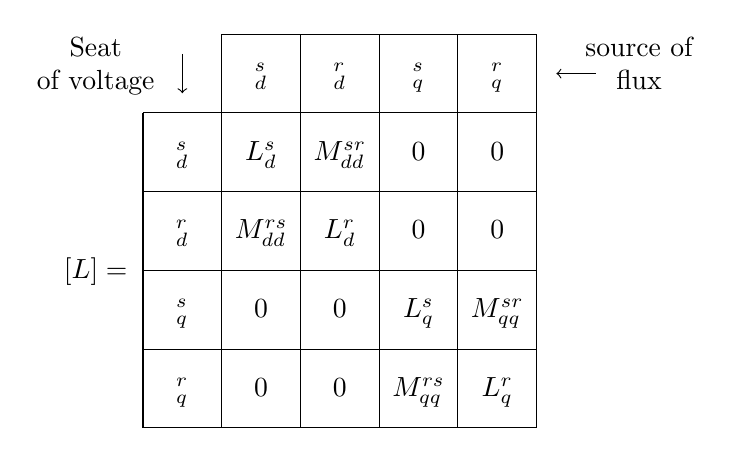
\begin{tikzpicture} [anchor = base, baseline =0pt]
		\draw (0,0)--(5,0) (0,1)--(5,1) (0,2)--(5,2) (1,3)--(5,3) (0,-1)--(5,-1) (0,-2)--(5,-2);
		\draw (0,-2)--(0,2) (1,-2)--(1,3) (2,-2)--(2,3) (3,-2)--(3,3) (4,-2)--(4,3) (5,-2)--(5,3);
		\draw (0.5,-1.6) node{$_q^r$} +(0,1) node{$_q^s$} +(0,2) node{$_d^r$} +(0,3) node{$_d^s$};
		\draw (1.5,-1.6) node{0} +(0,1) node{0} +(0,2) node{$M_{dd}^{rs}$} +(0,3) node{$L_d^s$}+(0,4) node{$_d^s$};
		\draw (2.5,-1.6) node{0} +(0,1) node{0} +(0,2) node{$L_{d}^{r}$} +(0,3) node{$M_{dd}^{sr}$}+(0,4) node{$_d^r$};
		\draw (3.5,-1.6) node{$M_{qq}^{rs}$} +(0,1) node{$L_q^s$} +(0,2) node{0} +(0,3) node{0}+(0,4) node{$_q^s$};
		\draw (4.5,-1.6) node{$L_q^r$} +(0,1) node{$M_{qq}^{sr}$} +(0,2) node{0} +(0,3) node{0}+(0,4) node{$_q^r$};
		\draw (-0.6,-0.1) node{$[L] =$};
		\draw [align = center,->](-0.6, 2.3) node{Seat\\of voltage} (0.5,2.75)--(0.5, 2.25);
		\draw [align = center,->](6.3, 2.3) node{source of\\flux} (5.75,2.5)--(5.25,2.5);
	\end{tikzpicture}
\end{equation}

The matrix contains mutual inductance coefficients forming equal pairs
\begin{align*}
	M_{dd}^{sr} & = M_{dd}^{rs} \\
	M_{qq}^{sr} & = M_{qq}^{rs}
\end{align*}
For a salient-pole machine
\begin{equation*}
	L_d^s \neq L_q^s , \quad L_d^r \neq L_q^r \text{and} M_{dd}^{sr} \neq M_{qq}^{sr}
\end{equation*}
as the $d$-axis and $q$-axis permeances are different. The corresponding inductances are equal for a machine with zero saliency.

\vspace{2em}

\noindent (b) \emph{The rotational coefficient matrix} $[G]$\\
The $[G]$ matrix in general form
\begin{equation}
	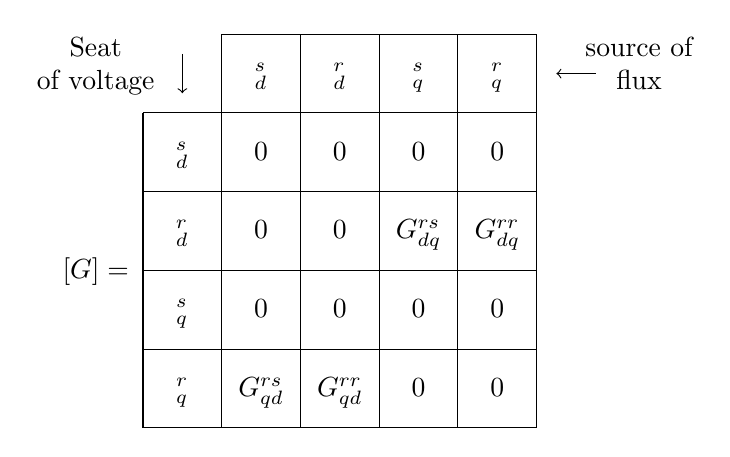
\begin{tikzpicture} [anchor = base, baseline =0pt]
		\draw (0,0)--(5,0) (0,1)--(5,1) (0,2)--(5,2) (1,3)--(5,3) (0,-1)--(5,-1) (0,-2)--(5,-2);
		\draw (0,-2)--(0,2) (1,-2)--(1,3) (2,-2)--(2,3) (3,-2)--(3,3) (4,-2)--(4,3) (5,-2)--(5,3);
		\draw (0.5,-1.6) node{$_q^r$} +(0,1) node{$_q^s$} +(0,2) node{$_d^r$} +(0,3) node{$_d^s$};
		\draw (1.5,-1.6) node{$G_{qd}^{rs}$} +(0,1) node{0} +(0,2) node{0} +(0,3) node{0}+(0,4) node{$_d^s$};
		\draw (2.5,-1.6) node{$G_{qd}^{rr}$} +(0,1) node{0} +(0,2) node{0} +(0,3) node{0}+(0,4) node{$_d^r$};
		\draw (3.5,-1.6) node{0} +(0,1) node{0} +(0,2) node{$G_{dq}^{rs}$} +(0,3) node{0}+(0,4) node{$_q^s$};
		\draw (4.5,-1.6) node{0} +(0,1) node{0} +(0,2) node{$G_{dq}^{rr}$} +(0,3) node{0}+(0,4) node{$_q^r$};
		\draw (-0.6,-0.1) node{$[G] =$};
		\draw [align = center,->](-0.6, 2.3) node{Seat\\of voltage} (0.5,2.75)--(0.5, 2.25);
		\draw [align = center,->](6.3, 2.3) node{source of\\flux} (5.75,2.5)--(5.25,2.5);
	\end{tikzpicture}
\end{equation}

It is seen that $G$ coefficients are only obtained for pseudo-stationary rotor coils. Coils acting as flux sources may be stator or pseudo-stationary rotor coils.

The significance of the $G$ coefficients is determined from
\begin{equation*}
	G_{rs} = -M_m \sin \theta_r
\end{equation*}

The value of $M_m$ is the coupling obtained when the axis of the seat of voltage coil is imagined to be aligned with the axis of the source of flux coil.

Coefficients with stator coils as the source of flux
\begin{align*}
	G_{dq}^{rs} &= - M_{qq}^{rs} \sin \Big (+\frac{\pi}{2}\Big) = -M_{qq}^{rs}\\
	G_{qd}^{rs} &= - M_{dd}^{rs} \sin \Big (-\frac{\pi}{2}\Big) = -M_{dd}^{rs}
\end{align*}

Coefficients involving two pseudo-stationary coils 
\begin{align*}
	G_{dq}^{rr} & =-M_{qq}^{rr} \sin \Big( +\frac{\pi}{2} \Big) = -M_{qq}^{rr}\\
	G_{qd}^{rr} & =-M_{dd}^{rr} \sin \Big( -\frac{\pi}{2} \Big) = -M_{dd}^{rr}\\
	M_{qq}^{rr} & = \sqrt{L_q^r L_q^r} = L_q^r \\
	M_{dd}^{rr} & = \sqrt{L_d^r L_d^r} = L_d^r
\end{align*}

Substituting the above inductance coefficients in (5.81)
\begin{equation}
	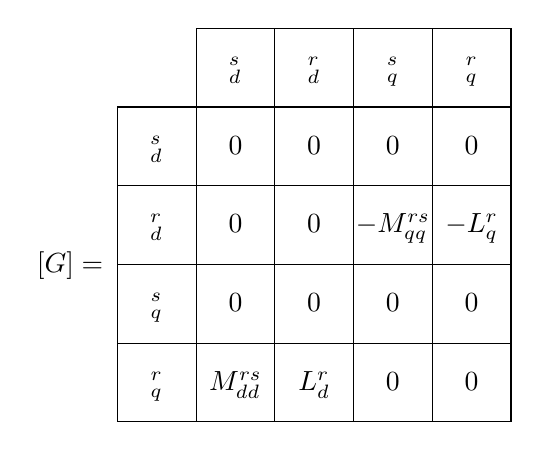
\begin{tikzpicture} [anchor = base, baseline =0pt]
		\draw (0,0)--(5,0) (0,1)--(5,1) (0,2)--(5,2) (1,3)--(5,3) (0,-1)--(5,-1) (0,-2)--(5,-2);
		\draw (0,-2)--(0,2) (1,-2)--(1,3) (2,-2)--(2,3) (3,-2)--(3,3) (4,-2)--(4,3) (5,-2)--(5,3);
		\draw (0.5,-1.6) node{$_q^r$} +(0,1) node{$_q^s$} +(0,2) node{$_d^r$} +(0,3) node{$_d^s$};
		\draw (1.5,-1.6) node{$M_{dd}^{rs}$} +(0,1) node{0} +(0,2) node{0} +(0,3) node{0}+(0,4) node{$_d^s$};
		\draw (2.5,-1.6) node{$L_{d}^{r}$} +(0,1) node{0} +(0,2) node{0} +(0,3) node{0}+(0,4) node{$_d^r$};
		\draw (3.5,-1.6) node{0} +(0,1) node{0} +(0,2) node{$-M_{qq}^{rs}$} +(0,3) node{0}+(0,4) node{$_q^s$};
		\draw (4.5,-1.6) node{0} +(0,1) node{0} +(0,2) node{$-L_{q}^{r}$} +(0,3) node{0}+(0,4) node{$_q^r$};
		\draw (-0.6,-0.1) node{$[G] =$};
		%\draw [align = center,->](-0.6, 2.3) node{Seat\\of voltage} (0.5,2.75)--(0.5, 2.25);
		%\draw [align = center,->](6.3, 2.3) node{source of\\flux} (5.75,2.5)--(5.25,2.5);
	\end{tikzpicture}
\end{equation}

Combining the results obtained in (5.80) and (5.82), substituting in the general voltage equation
\begin{equation*}
	[v] = \{[R] + [L]p+\omega_r[G]\}[i]
\end{equation*}
gives the complete impedance matrix for a four-coil, primitive machine, Fig. 5.18.
\begin{equation}
	\begin{bmatrix}
		v_d^s \\ v_d^r \\ v_q^s \\ v_q^r
	\end{bmatrix}
	=
	\begin{bmatrix}
		(R_d^s + L_d^s p) & M_{dd}^{rs}p & 0 & 0\\
		M_{dd}^{rs}p & (R_d^r + L_d^r p) & -\omega_r M_{qq}^{rs} &-\omega_r L_q^r \\
		0 & 0 & (R_q^s + L_q^s p) & M_{qq}^{rs} p \\
		\omega_r M_{dd}^{rs} & \omega_r L_{d}^{r} & M_{qq}^{rs} p & (R_q^r + L_q^r p)
	\end{bmatrix}
	\begin{bmatrix}
		i_d^s \\ i_d^r \\ i_q^s \\ i_q^r
	\end{bmatrix}
\end{equation}
\subsection{Torque and power}

Substituting (5.82) in (5.74)
\begin{equation}
	T_e = (\text{pole-pairs})
	\begin{bmatrix}
		i_d^s & i_d^r &i_q^s & i_q^r
	\end{bmatrix}
	\begin{bmatrix}
		0 & 0 & 0 & 0 \\
		0 & 0 & -M_{qq}^{rs} & -L_q^r \\
		0 & 0 & 0 & 0 \\
		M_{dd}^{rs} & L_d^r & 0 & 0 
	\end{bmatrix}
	\begin{bmatrix}
		i_d^s \\  i_d^r \\ i_q^s \\ i_q^r
	\end{bmatrix}
\end{equation}
Expanding and collecting terms
\begin{equation}
	T_e = (\text{pole-pairs}) [M_{dd}^{rs} i_d^s i_q^r - M_{qq}^{rs} i_q^s i_d^r + (L_d^r  - L_q^r)i_d^r i_q^r]
\end{equation}
The torque component in $(L_d^r - L_q^r)$ is only present in salient-pole machines and is called saliency-torque. The remaining torque components, which define the electromagnetic torque for a uniform air-gap, are described as cylindrical torques. It will be noted that the cylindrical torque components comprise a positive motoring term and a negative generating term; the sum of all such terms determines the machine action, motor, or generator.

The total internal electrical power developed by the machine
\begin{equation}
	P_e = \frac{\omega_r}{(\text{pole-pairs})} T_e
\end{equation}
\begin{equation}
	P_e = \omega_r [M_{dd}^{rs} i_d^s i_q^r - M_{qq}^{rs} i_q^s i_d^r + (L_d^r  - L_q^r)i_d^r i_q^r]
\end{equation}

An alternative method of deriving (5.85) is to consider the torque exerted of each pseudo-stationary coil by all coils at right-angles.
\chapter{D.C.\ and crossfield machines}
The physical arrangement of a d.c.\ or crossfield machine is identical to the primitive machine. The rotating commutator winding has one or more brush-pairs on orthogonal axes and stator coils are on the same orthogonal axes. The equation developed in chapter 5 for a primitive machine are directly applicable for these types of machines.
\section{General analysis}
Machine voltage and torque equations my be written down by inspection when the ideas and rules in chapter 5 are understood. For convenience, a two pole machine is always schematically shown although the equations apply for any number of pole-pairs.
Consider a machine with one brush-pair on the quadrature-axis and two direct-axis stator coils as shown in Fig. 6.1. The voltage and electromagnetic torque equations are:

\begin{equation}
	\begin{bmatrix}
        v_d^{s1}\\[2ex] v_d^{s2}\\[2ex] v_q^{r1}
	\end{bmatrix} =
    \begin{bmatrix}
        (R_d^{s1} + L_d^{s1}p) & M_{d}^{s1}{}_{d}^{s2} p & 0 \\[2ex]
        M{_d^{s2}{}_d^{s1}} & (R_d^{s2} + L_d^{s2}p) & 0 \\[2ex]
        \omega_r G_{q}^{r1}{}_d^{s1} & \omega_r G_{q}^{r1}{}_d^{s2} & (R_q^r1{} + L_q^{r1}p)
    \end{bmatrix}
    \begin{bmatrix}
        i_d^{s1} \\[2ex] i_d^{s2} \\[2ex] i_q^{r1}
    \end{bmatrix}
	\label{}
\end{equation}
\begin{equation}
    T_e = (\text{pole-pairs})[i_q^{r1}(G_q^{r1}{}_d^{s1} i_d^{s1} + G_q^{r1}{}_d^{s2} i_d^{s2})]
    \label{}
\end{equation}

The rotational inductance ($G$) coefficients mat be replaced by transformer inductance ($M$) coefficients as described in section 5.5.

\begin{equation}
    \begin{bmatrix}
        v_d^{s1}\\[2ex] v_d^{s2}\\[2ex] v_q^{r1}
	\end{bmatrix} =
    \begin{bmatrix}
        (R_d^{s1} + L_d^{s1}p) & M_{d}^{s1}{}_{d}^{s2} p & 0 \\[2ex]
        M{_d^{s2}{}_d^{s1}} & (R_d^{s2} + L_d^{s2}p) & 0 \\[2ex]
        \omega_r M_{d}^{r1}{}_d^{s1} & \omega_r M_{d}^{r1}{}_d^{s2} & (R_q^r1{} + L_q^{r1}p)
    \end{bmatrix}
    \begin{bmatrix}
        i_d^{s1} \\[2ex] i_d^{s2} \\[2ex] i_q^{r1}
    \end{bmatrix}
    \label{}
\end{equation}

\begin{equation}
    T_e = (\text{pole-pairs})[i_q^{r1}(M_d^{r1}{}_d^{s1} i_d^{s1} + M_d^{r1}{}_d^{s2} i_d^{s2})]
    \label{}
\end{equation}
Assuming a mechanical damping coefficient $D$ proportional to speed, the torque balance equation is.

\begin{equation}
    T_m + T_e = J p \omega_m + D \omega_m
    \label{}
\end{equation}
where, as previously, suffix $m$ refers to a mechanical quantity and $J$ is the polar moment of inertia.

The general equations (6.3) to (6.5) apply for steady-state or transient performance. For steady-state operation the derivative terms are zero and the equations are considerably simplified.

For simultaneous changes of current and speed the solution of the equations may be extremely formidable, see Section 6.4.3.
\noindent \textit{Simplified notation} In the previous chapter each primitive coil is identified by two letters and a number. With a particular machine arrangement it is more convenient to use a single letter to identify a winding, especially with d.c.\ and crossfield machines in which primitive coils correspond to actual windings.

For example, a coil designated $f$ has resistance $r_f$, self-inductance $L_f$, and its mutual inductance with a coil $s$ is $M_{sf}$.

\section{D.C.\ machine steady state analysis}
D.C.\ machines have one or more stator windings for the required load characteristic. Additional stator windings are included to give satisfactory commutation.

\subsection{Field windings} The main stator or field windings are wound on salient poles. Coils may be connected:
\begin{enumerate}[label = (\alph*)]
    \item in series with the rotor or armature winding, \\
    i.e.\ \textit{a series field}
    \item[or \stepcounter{enumi} (\alph{enumi})] energized from a separate d.c.\ supply, \\
    i.e.\ a \textit{separately-excited field}
    \item[or \stepcounter{enumi} (\alph{enumi})] across the armature brush-pair,\\
    i.e.\ a \textit{shunt field.}
\end{enumerate}
A d.c.\ motor with a shunt winding is identical to a separately-excited machine as in both cases the winding is energized from the supply voltage.

With a shunt generator, the simplifying assumption of a linear flux/current relationship is not justified as the open-circuit voltage is limited only by magnetic saturation. The analysis of this machine therefore requires a more realistic treatment, see Section 6.2.4.
A \textit{compound machine} has a series field together with a shunt or separately-excited field winding. The following analysis is for a compound machine with series and separately-excited windings.
\subsection{Compound machine analysis} Figure 6.2(a) shows the primitive coil arrangement for a compound machine. For simplicity, the armature and the series and separately-excited fields are designated $a$, $s$ and $f$, respectively. The primitive voltage equations are,

\begin{equation}
    \begin{bmatrix}
        v_d^{s2}\\[2ex] v_d^{s1}\\[2ex] v_q^{r1}
	\end{bmatrix} =
    \begin{bmatrix}
        (R_f + L_f p) & M_{fs} p & 0 \\[2ex]
        M_{sf} & (R_s + L_s p) & 0 \\[2ex]
        \omega_r M_{af} & \omega_r M_{as} & (R_a + L_a p)
    \end{bmatrix}
    \begin{bmatrix}
        i_d^{s2} \\[2ex] i_d^{s1} \\[2ex] i_q^{r1}
    \end{bmatrix}
    \label{}
\end{equation}

The field coils may be connected to give m.m.f.s in the same sense or in opposition to each other, and are termed either \textit{cumulative connected} or \textit{differential connected} windings, respectively. The two alternative connections for a machine in the motoring mode are shown in Figs.\ 6.2(b) and 6.2(c).
Reversal of the armature current also reverses the series field, and a differential connected motor operates as a cummulative connected generator. Similarly, a cumulative connected motor operates as a differential connected generator.

Establishing relationships between the primitive and the actual machine currents and voltages,
\begin{align*}
    i_q^{r1} & = i_a & v_q^{r1} & = v_a \\[2ex]
    i_d^{s1} & = \pm i_a & v_d^{s1} & = v_s \\[2ex]
    i_d^{s2} & = i_f & v_d^{s2} & = v_f
\end{align*}

In all cases the current $i_a$ is shown entering coil $a$ at the dot. For motor action,$i_a$ is a positive quantity and for generator action is a negative quantity.

The armature circuit voltage $V=v_a\pm v_s$, thus
\begin{equation*}
    V=v_q^{r1} \pm v_d^{s1}
    \label{}
\end{equation*}

Substituting in (6.6) for the primitive voltages and currents, combining $v_q^{r1}$ and $v_d^{s1}$ and writing $R = R_a + R_s$, $L = L_a + L_s$,

\begin{equation}
    \begin{bmatrix}
        v_f \\[2ex] V
    \end{bmatrix} =
    \begin{bmatrix}
        (R_f +F_f p) & \pm M_{sf} p \\[2ex]
        (\omega_r M_{af} \pm M_{sf} p) & (R + L p \pm \omega_r M_{as})
    \end{bmatrix}
    \begin{bmatrix}
        i_f \\[2ex] i_a
    \end{bmatrix}
    \label{}
\end{equation}

The electromagnetic torque equation is,
\begin{equation*}
    T_e = (\text{pole-pairs})[i_q^{r1} i_d{s2} M_{af} + i_q^{r1} i_d^{s1} M_{as}]
\end{equation*}
Substituting for actual currents,
\begin{equation}
    T_e = (\text{pole-pairs})[i_a M_{af} i_f \pm i_a^{2} M_{as}]
    \label{}
\end{equation}

The alternative sign $\pm$ is positive for a cumulative connected motor and a differential connected generator, and for a differential connected motor and a cummulative connected generator.

\subsection{Steady-state analysis} The steady-state operation of a compound machine is determined from the general performance equations. By omitting the appropriate winding from the current results for the compound machine, steady-state solutions for series and separately-excited machines are readily obtained.

\subsubsection{Compound machine} With constant speed and current values the $p \omega_r$ and $p i$ terms are zero, and (6.7), (6.8) and (6.5) may be written,
\begin{align}
    V & =\omega_r M_{af} I_f + (R \pm \omega_r M_{as}) I_a \\[2ex]
    T_e & = (\text{pole-pairs})[I_a M_{af} i_f \pm I_a^2 M_{as}] \\[2ex]
    T_m + T_e & = D \omega_m
\end{align}

Typical characteristics are shown for a compound machine in Fig. 6.3. A \textit{level-compounded} generator has  no voltage regulation.

\noindent In practice, saturation of the magnetic circuit increases the voltage regulation at high load currents and the term level-compounded describes a generator with zero voltage regulation at full load.

\subsubsection{Series machine} Omitting the separately-excited winding gives the steady-state equations for a series motor
\begin{align}
    V & = (R + \omega_r M_{as}) I_a\\[2ex]
    T_e & = (\text{pole-pairs})(I_a^2 M_{as})
    \label{}
\end{align}
The characteristics for a series motor, Fig. 6.4.\ show a high starting torque and the danger of running the machine on no-load. The series generator is seldom employed.

\subsubsection{\itshape\/Separately-excited machine or shunt motor} The steady-state equations are:
\begin{align}
    V & = R_a I_a + \omega_r M_{af} I_f\\[2ex]
    T_e & = (\text{pole-pairs})(I_a M_{af} I_f)
    \label{}
    \label{}
\end{align}

Typical characteristics are shown in Fig. 6.5.

\subsection{Shunt generator} The assumption made in the previous work may give raise to appreciable errors in analysing the performance of d.c.\ machines. However, the ability to derive and solve general equations for both steady-state and transient behaviour often justifies these assumptions. With these simplifying assumptions the performance of the shunt generator cannot be determined. The analysis of this machine requires a more realistic approach employing the
flux/excitation m.m.f.\ characteristic.
\subsubsection{Actual characteristics} The field current for a shunt generator is supplied by the armature voltage, see Fig. 6.6. With the armature rotating the residual flux in the stator poles generates a voltage across the brush-pair which drives current through the field winding increasing the pole flux, and hence, the armature voltage. The voltage continues to rise in a fairly linear manner with field current and the machine is said to self-excite. When the magnetic circuit of the pole flux
begins to saturate, the output voltage does not increases as rapidly as previously, see Fig. 6.7. A point is reached at which the voltage characteristic cuts the field resistance line and this corresponds to the open-circuit voltage of the machine.

Two necessary conditions for self-excitation are,
\begin{enumerate}[label= (\alph*)]
    \item the residual flux is in the \textit{correct sense}, i.e., field current due to rotational voltage reinforces the residual flux of the stator poles; and
    \item the slope of the field resistance line is sufficiently low to intersect the voltage characteristic at a reasonable value above the knee of the curve.
\end{enumerate}
For a given speed the \textit{critical field resistance} is the maximum value of field circuit resistance at which self-excitation occurs. With a given value of field circuit resistance there is a  \textit{critical speed} below which the machine fails to excite. The sudden short-circuit of an energized shunt generator reduces the excitation to zero and the steady-state value of short-circuit current, due only to residual pole flux, is small.

The solution of shunt generator problems requires graphical methods unless the magnetization characteristic can be expressed as an analytic function of the field current.

\subsubsection{Method of analysis} The non-linear voltage characteristic of a shunt generator, Fig. 6.7, may be represented wit reasonable accuracy by two linear parts of different slope as Fig. 6.8.

With \textit{incremental inductance coefficients} of $G_{af}^m$, $M_{af}^m$ and $G_{af}^n$, $M_{af}^n$ for the two slopes, the rotational voltage term in the armature coil is given by

\begin{align*}
    i_{f1} \geq i_f > 0, \hspace{8em}\\
    \text{rotational voltage term} & =\omega_r G_{af}^m i_f \\
    & = \omega_r M_{af}^m i_f\\
    i_f > i_{f1}, \hspace{10em} &\\
    \text{rotational voltage term} & = \omega_r [G_{af}^m i_{f1} + G_{af}^n (i_f - i_{f1})] \\
    &=  \omega_r [M_{af}^m i_{f1} + M_{af}^n (i_f - i_{f1})]
\end{align*}

The voltage and torque equations in the operating region above the knee of the curve, part $n$, are

\begin{align}
    v & = (R_a + L_a p)i_a + \omega_r M_{af} i_f \\
    v_f = v & = (R_f + L_f p) i_f\\
    T_e & = (\text{pole-pairs})(M_{af} i_a i_f)
    \label{}
\end{align}

As a function of $i_f$,

\begin{equation*}
    M_{af} = M_{af}^n + \frac{i_{f1}(M_{af}^m - M_{af}^n)}{i_f}
\end{equation*}

Eliminating $i_f$ from (6.16) and (6.17),

\begin{equation}
    v = \frac{(R_a + L_a p) i_a + \omega_r i_{f1} (M_{af}^m - M_{af}^n)}{1 - \dfrac{\omega_r M_{af}^n}{R_f + L_f p}} 
    \label{}
\end{equation}

For steady-state operation,

\begin{equation}
    v = \frac{R_a i_a + \omega_r i_{f1}(M_{af}^m - M_{af}^n)}{1 - \dfrac{\omega_r M_{af}^n}{R_f}}
    \label{}
\end{equation}

Equations (6.19) and (6.20) are valid for operation in region $n$ only, corresponding to a range of field current $i_f \geq i_{f1}$.

\subsection{Compensating winding} A d.c.\ machine with a severely fluctuating load, e.g.\ a rolling mill motor, may flashover across the commutator segments due to the high voltages induced in the armature coils by the rapidly changing armature current. A flashover often results in severe damage as short-circuit current may flow along the breakdown path. The large voltages induced in the armature coils may be eliminated by including a \textit{compensating winding} in the machine.

The voltage induced between two adjacent commutator segments depends on the rate of flux-linkage with the armature coil connected to the segments. There is an induced voltage (nearly independent of load current) due to the main excitation flux (an $\omega_r M$ term). An additional induced voltage may appear due to a rapid change of armature current and, hence, self-linkage (an $L p i$ term).

The compensating winding, connected in series with the armature, produces an m.m.f.\ equal and opposite to that of the armature, see Fig. 6.9(a). A rapid change of load current produces negligible change of flux along the $q$-axis, inducing little voltage in the armature coils.

Representing a separately-excited machine with a compensating winding as a primitive machinem Fig. 6.9(b), the coil voltages are
\begin{equation}
    \begin{bmatrix}
        v_d^{s1} \\[2ex] v_q^{s1} \\[2ex] v_q^{r1}
    \end{bmatrix} = 
    \begin{bmatrix}
        (R_f + L_f p) & 0 & 0 \\[2ex]
        0 & (R_c + L_c p) & M_{ca} \\[2ex]
        \omega_r M_{af} & M_{ca} p & (R_a + L_a p)
    \end{bmatrix}
    \begin{bmatrix}
        i_d^{s1} \\[2ex] i_q^{s1} \\[2ex] i_q{r1}
    \end{bmatrix}
    \label{}
\end{equation}

Connecting the armature and compensating windings,
\begin{align*}
    &\text{armature current}  & i_a & = i_q^{r1} = -i_q^{s1} \\
    &\text{armature circuit voltage} & v & = v_q^{r1} - v_q^{s1}
    \label{}
\end{align*}
equation (6.21) may be written

\begin{equation}
    \begin{bmatrix}
        v_f \\[2ex] v
    \end{bmatrix} =
    \begin{bmatrix}
        (R_f + L_f p) & 0 \\[2ex]
        \omega_r M_{af} & (R_a + R_c) + (L_a + L_c -2 M_{ac})p
    \end{bmatrix}
    \begin{bmatrix}
        i_f \\[2ex] i_a
    \end{bmatrix}
    \label{}
\end{equation}

Equations (6.22) are identical to those for a separately-excited machine with an armature resistance and inductance of ($R_a + R_c$) and ($L_a + L_c - 2M_{ac}$), respectively. With equal turns on the armature and compensating windings,
\begin{equation*}
    L_a \bumpeq L_c \bumpeq M_{ac}
\end{equation*}
and the effective armature inductance ($L_a + L_c - 2M_{ac}$) is negligible.

With the compensating winding not extending to the interpolar regions, as shown in Fig. 6.9(a), i.e., restricted to the pole faces, the compensating winding inductance is less than the armature self-inductance and the effective armature inductance ($L_a + L_c - 2M_{ac}$) may not be negligible.

\subsection{Interpole windings}
Satisfactory commutator action requires the current in a coil undergoing commutation to reverse in the commutation period, see Fig. 6.10. An induced voltage, produced by changing self-flux in the coil, opposes the current change and may prevent complete current reversal in the time allowed for commutation.

The difficulty is overcome in all modern machines by fitting \textit{interpoles} to give practically spark-free commutation at all loads and speeds. Interpoles, located s their name suggest in the interpolar region, see Fig. 6.11(a), are connected in series with the armature winding and produces fluxed which induce voltages in the coils undergoing commutation. These voltages are approximately equal and opposite to the self-induced voltages and enable the current to reverse
completely in the commutation period. Both self-induced and interpole induced voltages are proportional to speed and armature current, hence correct compensation is achieved for all values of speed and load, including rotation in either direction.

The interpole acts as a compensating winding over a small angle and is sometimes termed a \textit{commutating pole} or \textit{compole}.

The analysis is identical for machines with interpoles or compensating windings. However, the inductance of a interpole winding, $L_i$, is small compared with the armature inductance, $L_a$, and the modified armature circuit inductance ($L_a + L_i - 2M_{ai}$) cannot be ignored.

Interpoles are necessary for a machine with a compensating winding restricted to the salient-pole faces but are not required for a compensating winding which extends over the interpolar regions.

\subsection{Starting}
With full voltage applied to a stationary d.c.\ machine, the armature current, limited only by the low resistance of the armature circuit, would be dangerously large. Consequently, d.c.\ motors are always started at reduced armature voltage. A common method is additional resistance  in series with the armature which can be gradually removed as the speed increases. Full field current is applied to shunt machines to provide maximum rotational voltage as soon as possible. A typical
starter resistor has several sections which are cut out in turn as the motor increases speed. The current rises to a maximum shortly after switching-on and decays slowly as the armature rotational voltage build up with speed. On cutting-out the first resistor section the current increases rapidly to a peak value and then decays again. This is repeated until all starting resistance is out of circuit. The resistor sections are designed to limit the current maxima to a suitable
value provided that sufficient time is allowed for the current to fall to a certain minimum level before the next section is cut out. The problem is considered in more detail in Section 6.4.

\section{Sudden short-circuit of a d.c.\ generator}
The voltage and torque equations describing the performance of a machine are completely general and apply to transient as well as steady-state behaviour. As an example of transient analysis consider the sudden short-circuit of a d.c.\ generator with differential series and separately-excited field windings. The voltage equations are identical to those derived in Section 6.2.1 for the cumulative compound motor represented schematically in Fig. 6.2(b)
\begin{equation}
    \begin{bmatrix}
        v_f \\[2ex] v
    \end{bmatrix} =
    \begin{bmatrix}
        (R_f + L_f p) & M_{sf} p \\[2ex]
        (M_{sf} p + \omega_r M_{af}) & (R + L p + \omega_r M_{as})
    \end{bmatrix}
    \begin{bmatrix}
        i_f \\[2ex] i_a
    \end{bmatrix}
    \label{}
\end{equation}
Assuming no change of speed, i.e.\ $\omega_r$ is constant, the simultaneous linear differential equations (6.23) are readily solved using Laplace transforms.

\subsection{Analysis for a machine on load}
Consider a short-circuit at time $t=0$ on the output terminals of a generator with differential series and separately-excited field windings. The field voltage $V_f$ and the speed $\omega_r$ are assumed constant.
\begin{align*}
    \text{Pre-fault conditions}, t < 0\\
    & \text{armature (and series field) current } &= \mathring{I}_a\\
    & \text{output voltage} & = \mathring{V}\\
    & \text{field current} & = \mathring{I}_f\\
    \text{Fault condition}, t \geq 0 \\
    & \text{armature current, time-dependent} & = i_a\\
    & \text{field current, time-dependent} & = i_f \\
    & \text{output voltage} & = 0
\end{align*}

Substituting initial conditions in the voltage equations (6.23)
\begin{equation}
    \mathring{V} = \omega_r M_{af} \mathring{I}_f + R \mathring{I}_a + \omega_r M_{as} \mathring{I}_a
    \label{}
\end{equation}
(\textit{Note:} the current $\mathring{I}_a$ will be a negative quantity as the machine is generating.)

Transforming (6.23) by Laplace to the $\mathbf s$ domain and including initial conditions,
\begin{align}
    \bar v_f & = (R_f + L_f \mathbf{s})\bar i_f - L_f \mathring I_f + M_{sf} \mathbf{s} \bar i_a - M_{sf} \mathring I_a \nonumber \\ %chktex 7
    \bar v & = (M_{sf} \mathbf{s} + \omega_r M_{af} )\bar \imath_f - M_{sf} \mathring I_f + (R + L \mathbf{s} + \omega_r M_{as})\bar i_a - L\mathring I_a %chktex 7
    \label{}
\end{align}

In matrix notation (6.25) may be written with the initial conditions grouped together,
\begin{multline}
    \begin{bmatrix}
        \bar v_f \\[2ex] \bar v
    \end{bmatrix} = 
    \begin{bmatrix}
        (R_f + L_f \mathbf{s} ) & M_{sf}\mathbf s  \\[2ex]
        (M_{sf} \mathbf{s} + \omega_r M_{af} ) & (R + L\mathbf{s}+\omega_r M_{as} )
    \end{bmatrix}
    \begin{bmatrix}
        \bar i_f \\[2ex] \bar i_a %chktex 7
    \end{bmatrix} \\
    - 
    \begin{bmatrix}
        L_f & M_{sf} \\[2ex]
        M_{sf} & L
    \end{bmatrix}
    \begin{bmatrix}
        \mathring I_f \\[2ex] \mathring I_a
    \end{bmatrix}
\end{multline}
With initial conditions transferred to the left-side,
\begin{equation}
    \begin{bmatrix}
        \bar v_f + L_f \mathring I_f + M_{sf} \mathring I_a \\[2ex]
        \bar v + M_{sf} \mathring I_f + L \mathring I_a
    \end{bmatrix}
    =
    \Bigg[ Z(\mathbf s)\Bigg]
    \begin{bmatrix}
        \bar i_f \\[2ex] \bar i_a %chktex 7
    \end{bmatrix}
    \label{}
\end{equation}
Now
\begin{equation*}
    \begin{array}{r@{\;=\;}ll}
        \bar v & 0 & \text{for } t \geq 0 \text{, machine short-circuited} \\
        \bar v_f & \dfrac{V_f}{\mathbf s} &\text{as } v_f \text{\ is constant.}
    \end{array}
\end{equation*}
Equation (6.27) may be written,
\begin{equation}
    \begin{bmatrix}
        \dfrac{V_f}{\textbf{s}} + L_f \mathring I_f + M_{sf} \mathring I_a \\[2ex]
        M_{sf} \mathring I_f + L \mathring I_a
    \end{bmatrix}
    =
    \Bigg[ Z(\textbf{s})\Bigg]
    \begin{bmatrix}
        \bar i_f \\ \bar i_a %chktex 7
    \end{bmatrix}
    \label{}
\end{equation}

The solution for the transient currents $i_a(t)$ and $i_f(t)$ may be obtained using inverse Laplace transforms.

\subsection{Solution for unloaded machine}
With $\mathring I_a =0$, (6.28) and (6.24) reduce to
\begin{equation}
     \begin{bmatrix}
        V_f/\textbf{s} + L_f \mathring I_f \\[2ex]
        M_{sf} \mathring I_f 
    \end{bmatrix}
    =
    \Bigg[ Z(\textbf{s})\Bigg]
    \begin{bmatrix}
        \bar i_f \\ \bar i_a %chktex 7
    \end{bmatrix}
    \label{}
\end{equation}
\begin{equation}
    \mathring V = \omega_r M_{af} \mathring I_f
    \label{}
\end{equation}
Combining (6.29) and (6.30) and eliminating $i_f$,

\begin{equation}
    \bar i_a = - \dfrac{(\mathring V/\mathbf s)(R_f + L_f \mathbf s)}{(R + \omega_r M_{as}+L \mathbf s)(R_f + L_f \mathbf s) - M_{sf} \textbf{s} ( M_{sf} \textbf{s} + \omega_r M_{af})} %chktex 7
    \label{}
\end{equation}
Writing $\tau$ for $L / (R + \omega_r M_{as})$ and $\tau_f$ for $L/R_f$ in (6.31),
\begin{multline}
    \bar i_a = - \dfrac{\mathring V(1-\textbf{s}\tau_f)}{\textbf{s}(R + \omega_r M_{as}) \bigg\{1 + \textbf{s} \bigg[\tau + \tau_f - \dfrac{\omega_r M_{af} M_{sf}}{R_f (R + \omega_r M_{as})} \bigg]} \\ %chktex 7
      + \textbf{s}^2 \bigg[\tau \tau_f - \dfrac{M_{sf}^2}{R_f(R + \omega_r M_{as})}\bigg]\bigg\}
    \label{}
\end{multline}

\begingroup
\setlength{\lineskip}{2pt} 
\noindent Now $\dfrac{M_{sf}}{R_f(R + \omega_r m_{af})}$ may be written $\dfrac{K_{sf}^2}{(R + \omega_r M_{as}) R_f}$ \\
\phantom{Now }$= \tau \tau_f k_{sf}^2 \dfrac{L_s}{L}$ where $k_{fs}$ is the coefficient of coupling.\\

\endgroup
\noindent Substituting in (6.32)
\begin{multline}
    \bar i_a = - \dfrac{\mathring V(1-\textbf{s}\tau_f)}{\textbf{s}(R + \omega_r M_{as}) \bigg\{1 + \textbf{s} \bigg[\tau + \tau_f - \dfrac{\omega_r M_{af} M_{sf}}{R_f (R + \omega_r M_{as})} \bigg]} \\ %chktex 7
    + \textbf{s}^2 \bigg[\tau \tau_f \bigg(1 - \dfrac{k_{sf}^2 L_s}{L}\bigg)\bigg]\bigg\}
    \label{}
\end{multline}
Expressed in partial fraction form
\begin{equation}
    \bar i_a = - \dfrac{\mathring V}{\textbf{s}(R + \omega_r M_{as})} \dfrac{(A^2 - B^2)(1 + \mathbf s \tau_f)}{(\mathbf s + A + B)(\textbf{s} + A - B)} %chktex 7
    \label{}
\end{equation}
where
\begin{equation}
    A = \dfrac{1}{2 \tau \tau_f \bigg(1 - \dfrac{k_{sf}^2 L_s}{L}\bigg)} \bigg[\tau_f + \tau - \dfrac{\omega_r M_{af} M_{sf}}{R_f (R + \omega_r M_{as})}\bigg]
    \label{}
\end{equation}
and
\begin{equation}
    B^2 = A^2 - \dfrac{1}{\tau \tau_f \bigg(1 - \dfrac{k_{sf}^2 L_s}{L}\bigg)}
    \label{}
\end{equation}
Expanding (6.34)
\begin{multline}
    \bar i_a = - \dfrac{\mathring V}{(R + \omega_r M_{as})}\bigg\{\dfrac{1}{\mathbf{s}} + \big(\dfrac{A-B}{2B}\bigg) \bigg[\dfrac{1 - (A + B)\tau_f}{\mathbf{s} + A + B}\bigg] \\ %chktex 7
    - \bigg(\dfrac{A+B}{2B}\bigg)\bigg[\frac{1 - (A - B)\tau_f}{\mathbf{s}+A-B}\bigg]\bigg\} 
    \label{}
\end{multline}
Transforming
\begin{multline}
    \bar i_a(t) = - \dfrac{\mathring V}{(R + \omega_r M_{as})} \bigg\{1 + \bigg( \dfrac{A-B}{2B}\bigg) [1 - (A + B) \tau_f]e^{-(A-B)t} \\%chktex 7 
    - \bigg(\dfrac{A - B}{2B}\bigg)[1 - (A - B)\tau_f]e^{-(A - B)t}\bigg\}
    \label{}
\end{multline}

\subsection{Simplified solution} In a typical compound machine the self-inductance of the weak series field is small compared with the armature self-inductance. The armature circuit time constant is small compared with the time constant of the separately-excited field winding; i.e.\ $L_a \gg L_s$ hence $(L_a + L_s) \gg L_s$, $L \gg L_s$, and $\tau_f \gg \tau$. Neglecting the relatively small values in (6.35) and (6.36)
\begin{align}
    A & \bumpeq \dfrac{1}{2 \tau \tau_f} \bigg[\tau_f - \dfrac{\omega_r M_{af} m_{sf}}{R_f (R + \omega_r M_{as})}\bigg] \\
    B^2 & \bumpeq \big[ A^2 - \dfrac{1}{\tau \tau_f} \bigg]
    \label{}
\end{align}
Now let
\begin{align}
    K & = 1 - \dfrac{\omega_r M_{af} M_{sf}}{\tau_f R_f (R + \omega_r M_{as})} \nonumber \\
    & = 1 - \dfrac{\omega_r M_{af} M_{sf}}{L_f (R + \omega_r M_{as})}
    \label{}
\end{align}
Substituting (6.41) and (6.39) and (6.40)
\begin{align*}
    A & \bumpeq \dfrac{K}{2 \tau} \\
    B^2 & \bumpeq \bigg[ \dfrac{K^2}{4 \tau^2} - \dfrac{1}{\tau \tau_f} \bigg]
\end{align*}
For a typical machine
\begin{equation*}
    \dfrac{K^2}{4 \tau^2} = \dfrac{1}{\tau \tau_f}
    \label{}
\end{equation*}
hence
\begin{equation}
    B \bumpeq A \bumpeq \dfrac{K}{2 \tau}
    \label{}
\end{equation}
Now
\begin{equation*}
    \dfrac{1}{\tau \tau_f} \bumpeq (A^2 + B^2) = (A + B)(A - B) \bumpeq \dfrac{K}{\tau} (A - B)
\end{equation*}
and
\begin{equation}
    (A - B) \bumpeq \dfrac{1}{K \tau_f}
    \label{}
\end{equation}
Substituting (6.42) and (6.43) in (6.38) gives
\begin{multline}
    i_a (t) \bumpeq - \dfrac{\mathring V}{(R + \omega_r M_{as})} \bigg\{ 1 + \dfrac{\tau}{K^2 \tau_f}\bigg[1 - \dfrac{K \tau_f}{\tau}\bigg] e^{(- K / \tau)t} \\
    - \bigg[1 - \dfrac{1}{K} \bigg]  e^{(-1 / K \tau_f)t} \bigg\}
\end{multline}
Let
\begin{equation}
    \tau' = \dfrac{\tau}{K} \quad \text{and} \quad \tau_f ' = K \tau_f
    \label{}
\end{equation}
Substituting (6.45) in (6.44)
\begin{equation}
    i_a (t) \bumpeq - \dfrac{\mathring V}{(R + \omega_r M_{as})} \bigg\{ 1 + \bigg[ \dfrac{\tau '}{\tau_f '} -\dfrac{1}{K} \bigg] e^{-t/\tau '} - \bigg[1 - \dfrac{1}{K} \bigg] e^{- t / \tau_f '} \bigg\}
    \label{}
\end{equation}
Now
\begin{equation*}
    \tau ' \ll \tau_f ' \quad \text{because} \quad \dfrac{\tau}{K} \ll K \tau_f
\end{equation*}
Neglecting the relatively small value in (6.46)
\begin{equation}
    i_a (t) \bumpeq - \dfrac{\mathring V}{(R + \omega_r M_{as})} \bigg\{ 1 + \dfrac{e^{-t/\tau'}}{K} -\bigg[ \dfrac{K-1}{K} \bigg] e^{-t/\tau_f '}\bigg\}
    \label{}
\end{equation}

Figure 6.12 shows typical short-circuit current against time characteristics for three different values of $K$ and a machine with $\tau'=0.0132$ second and $\tau_f' = 0.226$ second.

\subsection{Discussion} The example considered in the previous sections show how the short-circuit of a d.c.\ machine may be analysed. Simplifying assumptions, e.g., constant speed, are very necessary for analytical solutions to be readily obtained from the differential equations.

In actual machines, the large armature current on short-circuit causes heave saturation in parts of the magnetic circuit and appreciable errors occur in the solution as constant machine inductances are assumed. Delayed commutation, due to interpole saturation, has the effect of brush-shift which may be represented by a series coil on the $d$-axis. Rapid changes of armature current and flux induce eddy currents in the magnetic circuit which limit initial flux changes of non-laminated
iron and, consequently, the machine inductances for transient and steady-state conditions are of different value.

\section{D.C.\ motor transients}
The general voltage and torque equations may be used to analyse machine operation with transient load changes.

In general, a change of load on a d.c.\ motor alters the speed. With a sudden change of load torque the mechanical inertia of the machine prevents instantaneous speed change, in a similar manner to inductance preventing sudden change on an electrical circuit. With a sudden change of inertia, e.g.\ by engaging a flywheel, there is a rapid change of speed which can be represented for purposes of analysis as a step change.

\subsection{Mechanical time constant} Consider an unloaded d.c.\ machine at rest with a suddenly applied armature voltage. With suitable assumptions the build-up of speed is exponential and the machine has a \textit{mechanical time constant} which depends on the moment of inertia, the electrical parameters, and the field excitation.

A separately-excited motor, Fig. 6.13(a), with constant field current $I_f$ has the following general equations,
\begin{align}
    v_a & = (R_a + L_a p)i_a + \omega_r M_{af} I_f \\
    T_e & = (\text{pole-pairs})(i_a M_{af} I_f) \\
    T_m + T_e & = J p \omega_m + D \omega_m  
    \label{}
\end{align}

To obtain the required exponential expression for speed run-up, the armature inductance $L_a$ and the mechanical damping $D$ are assumed to be zero. The machine is unloaded, $T_m = 0$, and (6.48), (6.49) and (6.50) can be written,
\begin{align}
    v_a & = R_a i_a + \omega_m (\text{pole-pairs}) M_{af} I_f \\
    T_e & = (\text{pole-pairs})M_{af} I_f i_a = J p \omega_m
    \label{}
\end{align}

Eliminating $i_a$,
\begin{equation}
    v_a = \dfrac{R_a J p \omega_m}{(\text{pole-pairs}) M_{af} I_f} + (\text{pole-pairs}) \omega_m M_{af} I_f
    \label{}
\end{equation}
and
\begin{equation}
    \omega_m = \dfrac{v_a (\text{pole-pairs}) M_{af} I_f}{R_a J p + {(\text{pole-pairs})}^2 M_{af}^2 I_f^2}
    \label{}
\end{equation}

A constant armature voltage is suddenly applied at $t = 0$ to the machine initially at rest,
\begin{align*}
    t & < 0 & v_a & = 0 & \omega_m & = 0\\
    t & \ge 0 & v_a & = V_a
\end{align*}

Transforming (6.54) by Laplace,
\begin{align}
    \overline{\omega_m} & = \dfrac{V_a}{\mathbf{s}} \bigg[ \dfrac{(\text{pole-pairs}) M_{af} I_f}{{(\text{pole-pairs})}^2 M_{af}^2 I_f^2 + R_a J \mathbf{s}} \bigg] \nonumber \\
    & = \dfrac{V_a}{(\text{pole-pairs}) M_{af} I_f} \bigg[ \dfrac{1}{\mathbf{s}(1 + \tau_m \mathbf{s})}\bigg]
    \label{}
\end{align}
where
\begin{equation}
    \tau_m = \dfrac{R_a J}{{(\text{pole-pairs})}^2 M_{af}^2 I_f^2}
    \label{}
\end{equation}
Solving (6.55)

\begin{equation}
    \omega_m (t) = \dfrac{V_a}{(\text{pole-pairs}) M_{af} I_f} (1-e^{-t / \tau_m})
    \label{}
\end{equation}

Now $\dfrac{V_a}{(\text{pole-pairs}) M_{af} I_f}$ is the maximum speed $\omega_{m(\max)}$

\begin{equation}
    \omega_m(t) = \omega_{m(\max)} (1 - e^{-t / \tau_m})
    \label{}
\end{equation}

$t_m$ is called the \textit{mechanical time constant for run-up} of the machine.
Now
\begin{align}
    \tau_m & = \dfrac{R_a J}{{(\text{pole-pairs})}^2 M_{af}^2 I_f^2} \nonumber \\
    & = J \bigg[ \dfrac{V_a}{(\text{pole-pairs}) M_{af} I_f}\bigg] \bigg[\dfrac{R_a}{V_a (\textit{pole-pairs}) M_{af} I_f}\bigg] \nonumber \\
    \tau_m & = \dfrac{J \omega_{m(\max)}}{\text{starting torque}}
    \label{}
\end{align}

Hence, a simple expression is obtained for the mechanical time constant with mechanical damping and armature inductance neglected. Figure 6.13(b) illustrates the run-up speed and current characteristics.

\subsection{Starting transient} The armature of a d.c.\ motor is energized through resistance on starting, see Section 6.2.7. Consider the starting transient of a shunt motor. To simplify the solution it will be assumed that,
\begin{enumerate}[label= (\alph*)]
    \item the field current has a steady value $I_f$ before the armature circuit is energized,
    \item the armature self-inductance is small and may be neglected, and
    \item the machine is unloaded, $T_m = 0$, and mechanical damping is ignored.
\end{enumerate}

For an armature circuit resistance $R_m$,, which includes starting resistance, the machine equations are,
\begin{align}
    V & = i_a R_m + \omega_r M_{af} I_f \\
    T_e & = {(\text{pole-pairs})}(M_{af} I_f) = J p \omega_m
    \label{}
\end{align}
\subsubsection{\textit{Number of resistor section}} A relationship may be determined for the required number of starter sections. Let there be $(n - 1)$ sections, $n$ contact studs and a total starter resistance $R_n$ including armature resistance $R_a$, see Fig. 6.14. For each stud position armature current limits of $I_{a(\max)}$ and $I_{a(\min)}$ are assumed.

The following tabulated results are obtained using these limits in (6.60).

\begin{tabular}{llll}
    \begin{tabular}{c}
        Time \\ $t$ \\
    \end{tabular} &
    \begin{tabular}{c}
        Contact \\ stud \\
    \end{tabular} &
    \begin{tabular}{c}
        Speed \\ $\omega_r$ \\
    \end{tabular} &
        Supply Voltage $V$ \\
    0 &  $n$ & 0 & $I_{a(\max)} R_n$ \\
    $t_1$ & $n$ & $\omega_{m1}$ & $I_{a(\min)} R_n + \omega_{r1} M_{af} I_f$\\
    $t_1$ & $(n - 1)$ & $\omega_{m1}$ & $I_{a(\max)} R_{n-1} + \omega_{r1} M_{af} I_f$\\
    $t_2$ & $(n - 1)$ & $\omega_{m2}$ & $I_{a(\min)} R_{n-1} + \omega_{r2} M_{af} I_f$\\
    $t_2$ & $(n - 2)$ & $\omega_{m2}$ & $I_{a(\max)} R_{n-2} + \omega_{r1} M_{af} I_f$\\
    \vdots & \vdots & \vdots & \vdots \\
    $t_{n-1}$ & 2 & $\omega_{m(n-1)}$ & $I_{a(\min)} R_2 + \omega_{r(n-1)} M_{af} I_f$\\
    $t_{n-1}$ & 1 & $\omega_{m(n-1)}$ & $I_{a(\max)} R_a + \omega_{r(n-1)} M_{af} I_f$\\
\end{tabular}

Eliminating rotational voltage terms from pairs of equations of common angular speed,
\begin{equation}
    \dfrac{I_{a(\max)}}{I_{a(\min)}} = \dfrac{R_n}{R_{n-1}} = \dfrac{R_{n-1}}{R_{n-2}} = \cdots = \dfrac{R_2}{R_a}
    \label{}
\end{equation}

Multiplying all resistance ratios,
\begin{equation}
    {\bigg[\dfrac{I_{a(\max)}}{I_{a(\min)}}\bigg]}^{n - 1} = \dfrac{R_n}{R_a}
    \label{}
\end{equation}

Equations (6.62) and (6.63) enable the number of sections and section resistance values to be determined for prescribed limiting values of armature current.

\subsubsection{\textit{Run-up speed characteristic}} The speed change is exponential for the assumptions listed in Section 6.4.1.
From (6.58),
\begin{equation*}
    \omega_m = \omega_{m (\max)}(1 - e^{-t / \tau_m})
\end{equation*}

The maximum speed is independent of the armature resistance, as mechanical damping is neglected.

The values of $\tau_m$, given in (6.59), depends on the armature circuit resistance which now includes starter resistance. \par \smallskip
\begin{tabularx}{\textwidth}{l@{\enskip}ll}
    Let & $\tau_{m(n)}$ & be the time constant with $R_n$ in circuit \\
    & $\tau_{m(n-1)}$ & be the time constant with $R_{n-1}$ in circuit \\
    & $\tau_{m}$ & be the time constant with $R_{a}$ in circuit. \\
\end{tabularx}

Considering the times $t_1$, $t_2$, etc., defined previously
     %\intertext{$0<t<t_1, R_n$ in circuit,}
\begin{flalign}
    \omega_m (t) & = \omega_{m(\max)}[1 - e^{-t / \tau_{m(n)}] \\
    \omega_{m(\max)} & = 
\end{flalign}

\end{document}
